\documentclass{article}
\usepackage{a4wide}
\usepackage[english]{babel}
\usepackage{amsmath}
\usepackage{amssymb}
\usepackage{dsfont}
%\usepackage[dvips]{epsfig}
%\usepackage{graphicx}
\usepackage{fancyhdr}
\usepackage{listings}
\usepackage{nomencl}
\usepackage[pdftex]{graphicx}

\pagestyle{fancy}
\lhead{\footnotesize \parbox{11cm}{A.J. H\"ormer, E. Vontobel, A. Novacek}}
\rhead{\footnotesize {Plexos Project}}
\chead{\footnotesize {TET4135}}

\title{Report Plexos Project}
\author{Andreas Johann H\"ormer, Eva Vontobel, Adam Novacek}
\date{\today}

\begin{document}
\thispagestyle{empty}
\maketitle
\thispagestyle{empty}
%\\[5cm]
\begin{center}
TET4135 Energiplanlegging\\[3cm]
Lab group:
\begin{itemize}
\item Andreas Johann H\"ormer
\item Eva Vontobel
\item Adam Novacek\\[3cm]
\end{itemize}
Report delivered: \today\\[6cm]
FACULTY OF INFORMATION TECHNOLOGY, MATHEMATICS AND ELECTRICAL ENGINEERING\\
NORWEGIAN UNIVERSITY OF SCIENCE AND TECHNOLOGY
\end{center}
\thispagestyle{empty}
\newpage
\tableofcontents
\thispagestyle{empty}
\newpage
\listoffigures
\thispagestyle{empty}
\newpage
\section*{Abstract}
\thispagestyle{empty}

\newpage
\setcounter{page}{1}
\section{Introduction}
In this project we are modeling and analyzing a highly simplified version of the Nordic power system and its connection to continental Europe. The system consists of three nodes representing Norway, Sweden and Germany linked with transmission lines. Norway produces energy through two hydro plants, a wind power plant, and a gas plant. The annual demand in Norway is roughly 130 TWh. The annual demand in Germany is almost 550TWh covered with several coal, nuclear, gas and oil plants and two renewable consisting of solar and wind. Sweden has next to nuclear, coal, gas, oil, hydro and wind, a biopower plant to cover the demand of 145TWh. In a first part the main goal is to find the optimal operation plan for this system for the year 2014 and detect the impact of different weather conditions. In a second part the objective is to conduct Expansion planning with given investment options and evaluate the optimal approach. This report should clarify the influence of different weather conditions on an operation plan. The report also works with two different approaches for the expansion plan using  green certificate and emission taxes. The report deliver an insight to what is built, when and where and how this effects the prices, emissions and capacities.
\section{Theory}
\subsection{Methods used in the present work}
\subsubsection{Plexos}
\textit{Plexos for power systems} is a integrated graphical simulation software for short, medium and long time analysis of power systems\footnote{The version used for the analysis in the report was Plexos 6.3 x64 for Windows}. The possibility of price forecasting with respect to emissions and support mechanisms makes it possible to determine the optimal investment dates for power system expansion.\\
Plexos uses an object-oriented design, where generation units, regions, transmission lines, ..., are implemented as classes, instances of them are modeled as objects. The objects are combined using relationships and dependencies between them.
\subsubsection{MT Schedule}
The medium term schedule is a implemented simulation model based on a load duration curve analysis. The analysis can be done with weekly or monthly data and gives a full tabular and graphical representation of the generation units as well as the transmission lines. The medium term schedule is normally done for planning horizons of up to 2 years.
\subsubsection{Expansion planning}
The energy consumption in grids changes continuous. People are born, die or move to other places. Also the way of using energy changes. Energy-efficient lamps reduce the amount of power needed, at the same time electric cars appear. Due to this permanent changing of consumption a simulation of a very long time has to be done to find the optimal dates to invest in new transmission lines and generation units. The time periods for simulation are over a long time, a planning horizon of 20 years is quite common.\\
Generally the expansion planning is a three-dimensional problem. It has to be determined \textit{what} has to be built, \textit{when} and which \textit{size} it should have. The planning is done with dynamic programming, and can normally be reduced to a 2D- or even 1D-model due to known investment dates or given investment types. It is a static planning approach and can done in two different ways:
\begin{itemize}
\item marginal analysis in time\\
In this case the net benefit from year to year should be maximized. The calculation of net benefit is always done for the following year. The net benefit - calculated using the annuity - is planned as difference between fixed costs with and without investment. If the net benefit is positive, the investment should be done.
\item integral analysis in time\\
For this planning approach the net benefit over the whole analysis period should be maximized, while the time of investment is given as $t_0$. If the net benefit is positive, the investment should be done at $t_0$.
\end{itemize}
In practise these two planning approaches should be combined. The marginal analysis is used to simulate if the investment is profitable at $t_0$ or later, and the integral analysis for maximazing the net benefit over the whole period.
\subsection{The handling of intermittent resources}
Unlike fossil power plant, wind, solar and small hydro plants do not have fuels with fixed prices which could be used for an optimization. These intermittent resources are dependent on weather conditions. The flow in a river isn´t stable over the year and there is always the possibility of unexpected happenings. There is no chance to forecast the wind or the amount of sun for the next few years. Experienced data is important in a simulation with intermittent resources. The quality of experienced data is dependent on the amount of data available. In this project we use weekly inflow patterns for the small hydro plants and hourly profiles for the wind and solar plants. 
\subsection{The handling of reservoir hydro}
Calculating with reservoir hydro is not as straight forward as with thermal units because there are no fuel prices which could be used for an optimization. Even if the water to a reservoir comes for free, does not mean that it does not have a value. The quantity of water is limited. Often there are environmental regulations that need to be considered. For example fixed residual water flows. To calculate with a reservoir it is important to have information about the reservoir size (maximum and minimum capacities) and inflow patterns. The question with hydro reservoirs is: should we use the water right away or store it for later? If there is a large inflow, spillage can occur and the economic value will be zero. If the Inflow is very low, there is the risk of drainage.In that case the reservoir cannot produce enough energy to cover the demand. It is very difficult to forecast the conditions. In this project we work with different inflow scenarios in order to identify the influence of different reservoir levels to the optimal operation plan.
\subsection{Exchange between regions}
Power is a vital element that supports our modern lives. Power has to be available to any time at day and night. To cover the increasing demand and create a stable system transmission of power between countries has become more and more common. 
\subsubsection{Advantage}
The focus of power exchange is trade. Economic theory states that a perfectly free market is equal to the optimal use of resources. A common power market introduces free competition and increases stability\footnote{www.nordpoolspot.com/How-does-it-work/}. Available power capacities can be used more efficiently due to a larger region. Another advantage is that power can be produced on the most economic worthwhile region. For example is a wind power plant built in an offshore region better placed than in a region with lack of wind. This advantage leads to the fact that more power from different sources like hydro, thermal, wind and solar enters the grid. The market get more "liquid" and is not as depending on weather conditions anymore.  The price of power is determined according to supply and demand. A larger area often has a less labile demand which affects the prices in a positive way.
\subsubsection{Disadvantages}
If there is a unexpected peak demand or supply shortage in the common market, prices can get extremely volatile. The characteristics of such a price risk are highly dependent on the fundamentals of the market such as the mix of generation types. Another disadvantage is the risk of getting dependent on another country due to the fact that energy can be produced there cheaper. There is a risk of supply shortage if the political condition change.
%-------------------------------------------------------------------------------
% Investment initiatives
%-------------------------------------------------------------------------------
\subsection{Initiatives to increase investments for renewables}
The support of renewable energy sources has in the latest years more and more become an international issue. Global warming has pointed out the need of international and national laws and regulations.
\begin{itemize}
\item International\\
International laws and regulations try to follow the motto from the "Brundtland Commission": Think globally and act locally.  On the international level, there are two key documents. First there is the Rio Declaration, a statement of 27 principles upon which nations agreed to base their actions in dealing with environmental issues. And Second there is the Kyoto Protocol, an international agreement which commits its parties to set binding emission reduction targets. These documents introduce several mechanisms how to stimulate increased investments from renewable.
\item National (Norway)\\
Norway introduced the Energy Act to follow up with its obligations. The Energy Act states that all production, conversion, transmission, sales, distribution and consumption of different energy forms shall be done in a "social rational way". Together with Sweden developed Norway a market-based power system.
\end{itemize}

\subsubsection{Mechanisms}
\begin{itemize}
\item investment support\\
One time financial support to cover part of the investment costs.  The support is large enough to make the investment profitable. The support can be finetuned, eg. different support quantities can be applied. This means, that eg. for areas with less wind more investment support for wind power is done than in windy areas. This is done because when less wind occur, lower amounts of energy are produced and the less money is earned due to production.
\begin{itemize}
\item Advantages
\begin{itemize}
\item possibility of finetuning
\end{itemize}
\item Disadvantages
\begin{itemize}
\item requires much capital at beginning
\item no incentive to produce
\item limited security for investor
\item in case of fine tuning: much administration
\end{itemize}
\end{itemize}
\item Tendering\\
Auction for a certain amount of capacity which shall be installed. Won by the offers requiring the lowest support. This initiative is also done as investment support, but with a tendering procedure. Providers are asked for support bids, the cheapest one gets the support.
\begin{itemize}
\item Advantages
\begin{itemize}
\item competition between suppliers, therefore lower costs than investment support
\end{itemize}
\item Disadvantages
\begin{itemize}
\item same as investment support, but
\item less predictability
\item prone to corruption
\end{itemize}
\end{itemize}
\item Feed-in tariff\\
A fixed price for feeded kWh is payed for a predefined period.
\begin{itemize}
\item Advantages
\begin{itemize}
\item promotion of mid-term and long-term technologies
\item investment security for producer
\end{itemize}
\item Disadvantages
\begin{itemize}
\item possible risk of technology overfunding
\end{itemize}
\end{itemize}
\item Premium\\
Like feed-in tariff, but instead of a fixed price an additional amount per kWh is paid to the producer.
\begin{itemize}
\item Advantages
\begin{itemize}
\item market based
\end{itemize}
\item Disadvantages
\begin{itemize}
\item less certainty than feed-in tariff
\end{itemize}
\end{itemize}
\item Green certificates\\
This is a nordic system for supporting renewables. Some amount of certified energy has to be bought from energy suppliers, otherwise they are penalized. The intention is to build as much renewables as possible in short time. From 2020 new renewables are not certified any more, so the possibility to get enough certified power decreases and the risk of getting penalized increases.
\begin{itemize}
\item Advantages
\begin{itemize}
\item control of total amount of renewables
\item efficient market-based solution
\end{itemize}
\item Disadvantages
\begin{itemize}
\item less certainty than feed-in
\item complex
\item high administration costs
\end{itemize}
\end{itemize}
\end{itemize}

\section{Analysis}

%-------------------------------------------------------------------------------
% MT Schedule
%-------------------------------------------------------------------------------
\subsection{MT Schedule}
The medium term schedule is done for one year. Three different scenarios (low, normal, high inflow) to the reservoirs in Norway and Sweden are simulated. The different scenarios are described below.

%-------------------------------------------------------------------------------
% normal inflow scenario
%-------------------------------------------------------------------------------
\subsubsection{Normal inflow scenario}
For this case a normal inflow scenario was chosen. The inflow accords to the average inflow in a year in Norway and Sweden.
\paragraph{Optimal generation dispatch\\}
The optimal generation dispatch for normal inflow for Germany can be seen in figure \ref{fig:MTgenerationGnormal}. The generation dispatch for swedish generation units can be seen in figure \ref{fig:MTgenerationSnormal}, the norwegian dispatch is shown in figure \ref{fig:MTgenerationNnormal}.
\begin{itemize}
\item Germany\\
The nuclear power plants as well as the small coal power plant are running the whole year with full capacity for serving the base load. It can be obtained that in the winter is less solar power produced than in the summer, but more wind power is generated. The oil and small/medium gas generation units are hardly producing any power.
\item Sweden\\
The base load in Sweden is fully covered by nuclear and coal power. In summer some peak load is generated with small hydro, in winter the peak load is mainly covered with reservoir hydro. No power is produced with oil power plants, only small amount with gas generation.
\item Norway\\
In Norway more or less all power is produced by hydro power. In winter the power generation is mainly done with reservoir hydro, in summer about half of the produced energy is done with small hydro power. Some additional power is produced with wind generation, the installed gas power plant is producing no energy.
\end{itemize}
\begin{figure}[htbp]
\begin{center}
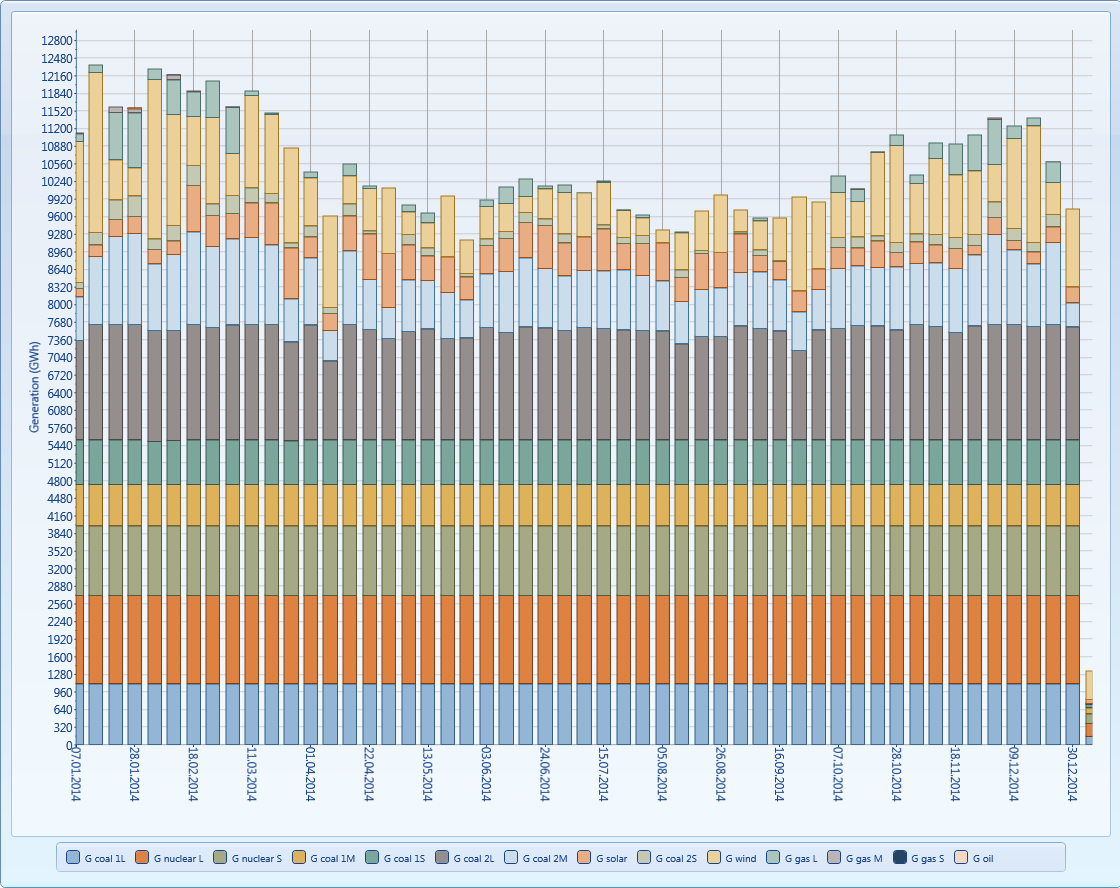
\includegraphics[width=13cm,keepaspectratio=true]{figures/MTgenerationG}
\caption{Optimal generation dispatch for Germany 2014 with normal inflow}
\label{fig:MTgenerationGnormal}
\end{center}
\end{figure}
\begin{figure}[htbp]
\begin{center}
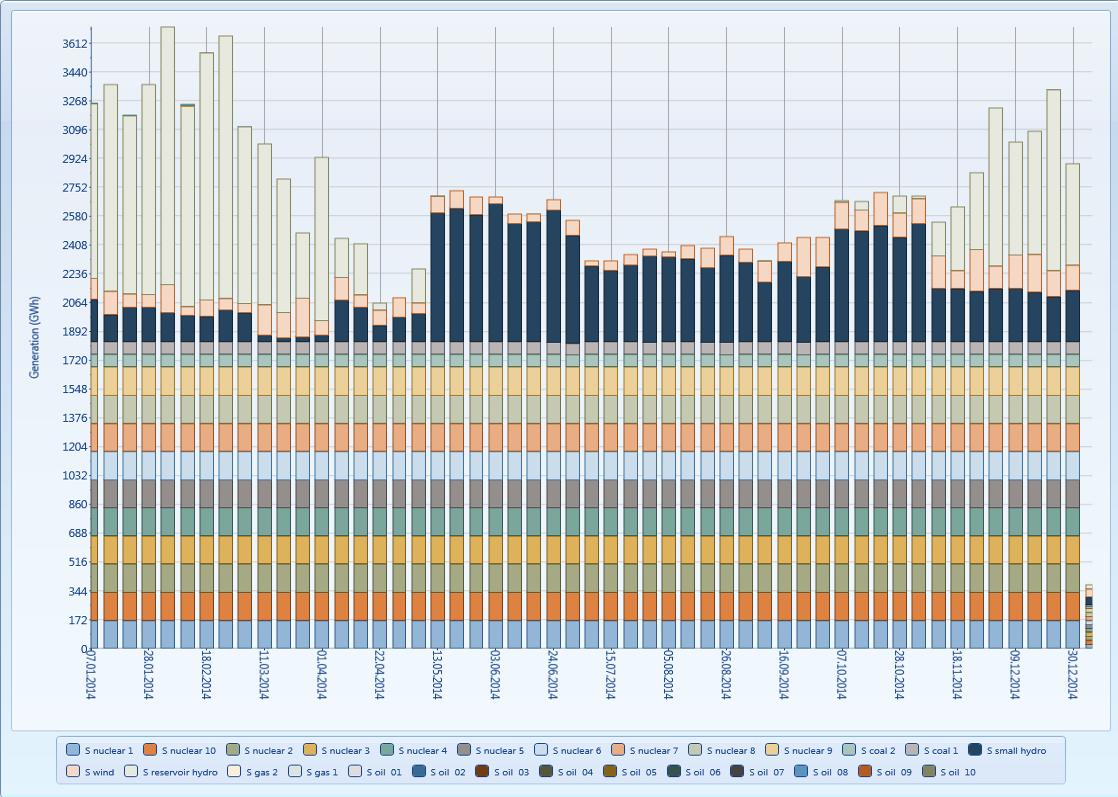
\includegraphics[width=13cm,keepaspectratio=true]{figures/MTgenerationS}
\caption{Optimal generation dispatch for Sweden 2014 with normal inflow}
\label{fig:MTgenerationSnormal}
\end{center}
\end{figure}
\begin{figure}[htbp]
\begin{center}
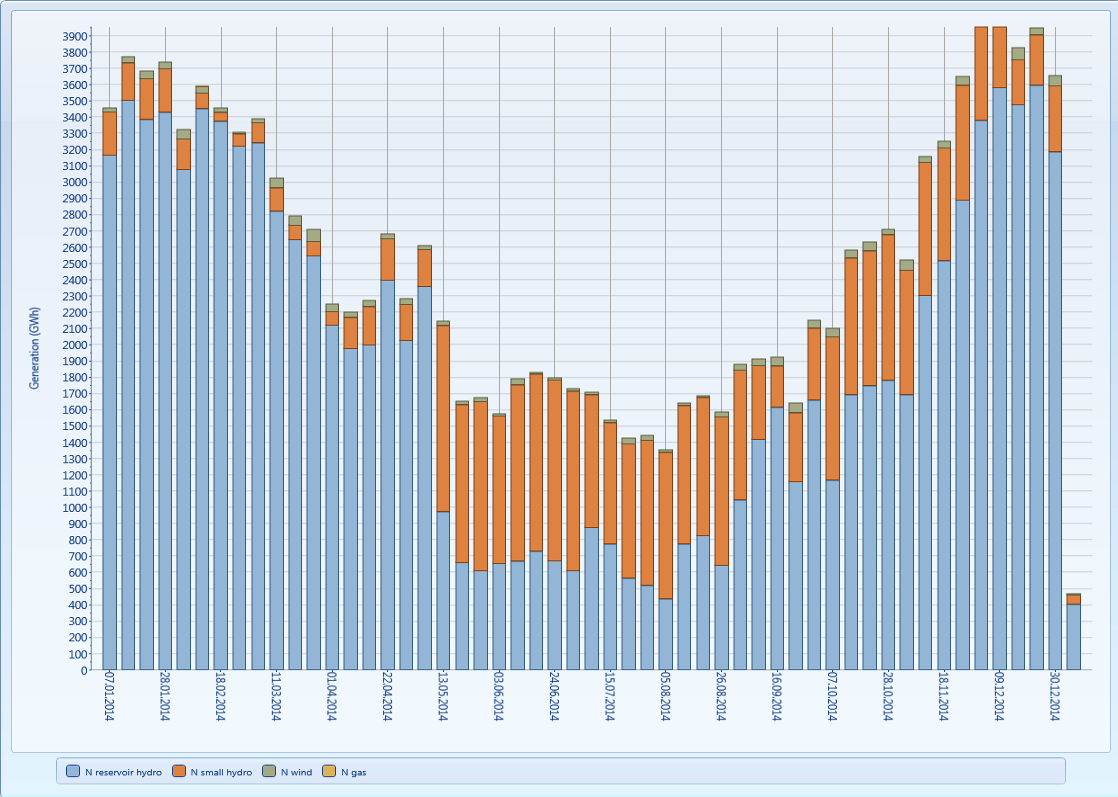
\includegraphics[width=13cm,keepaspectratio=true]{figures/MTgenerationN}
\caption{Optimal generation dispatch for Norway 2014 with normal inflow}
\label{fig:MTgenerationNnormal}
\end{center}
\end{figure}
\paragraph{Transmission\\}
The transmissions between the three countries Norway, Sweden and Germany is shown in figure \ref{fig:MTnodetransmissionnormal}. It is done not considering the flow direction, but the amount of power. Here it can be seen that most power flows between May and October. In winter there is very low flow between Norway and Sweden. The most continuous flow exists between Norway and Germany.
\begin{figure}[htbp]
\begin{center}
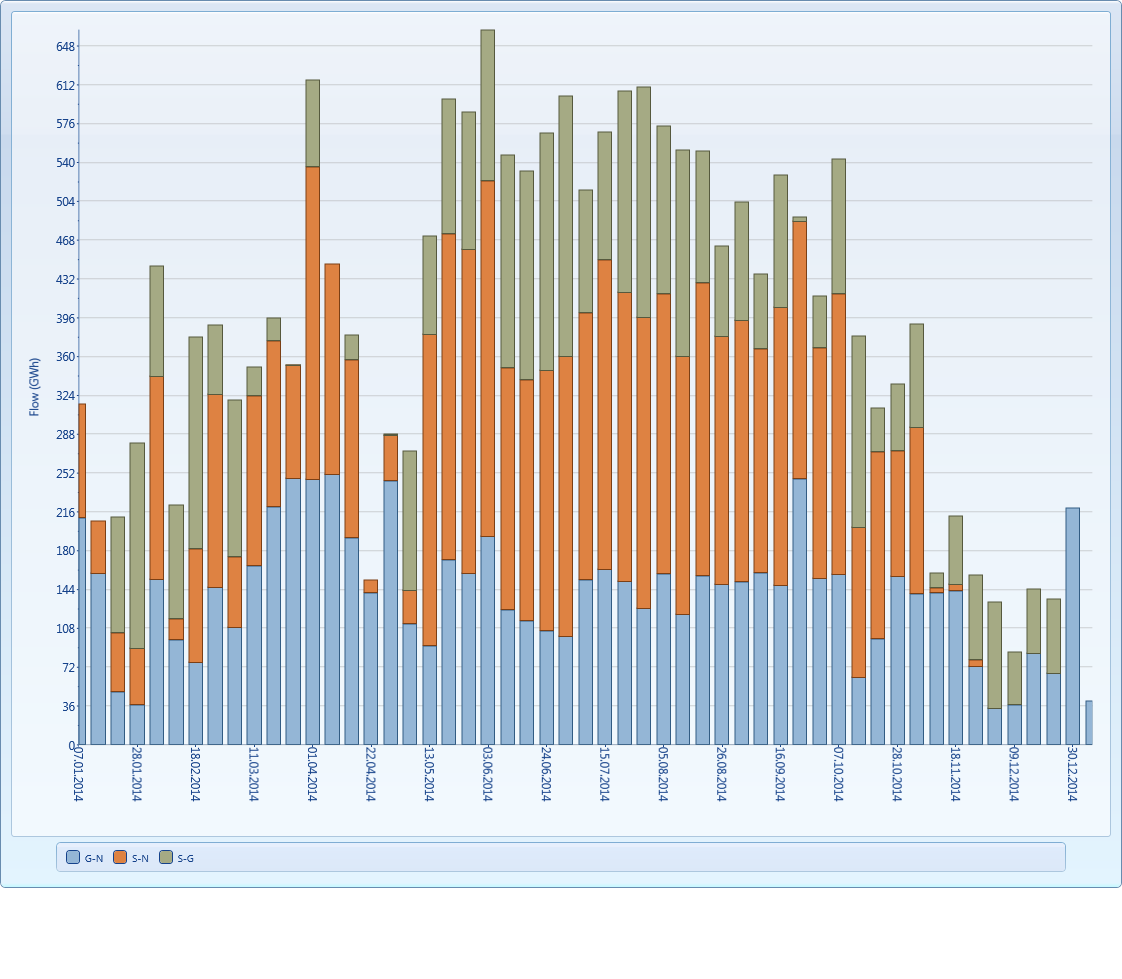
\includegraphics[width=13cm,keepaspectratio=true]{figures/MTnodetransmission}
\caption{Transmission between N/W/S with normal inflow}
\label{fig:MTnodetransmissionnormal}
\end{center}
\end{figure}
\paragraph{Emission\\}
The total emissions for all countries together can be seen in figure \ref{fig:MTemissionsnormal}. The emissions can be interpreted in following way:
\begin{itemize}
\item Norway: Due to the fact that most power installed is done with renewables (hydro power, wind power) and only some small amount of gas power, there are hardly and $CO_2$-emissions in Norway.
\item Sweden: Some renewable energy and a large amount of nuclear power lead to small $CO_2$-emissions. 
\item Germany: The biggest amount of the produced emissions are emitted from german power plants. Due to the fact that the base load is done with non-renewable energy, the emissions are mainly constant over the whole year, with some increases during the heating season.
\end{itemize}
\begin{figure}[htbp]
\begin{center}
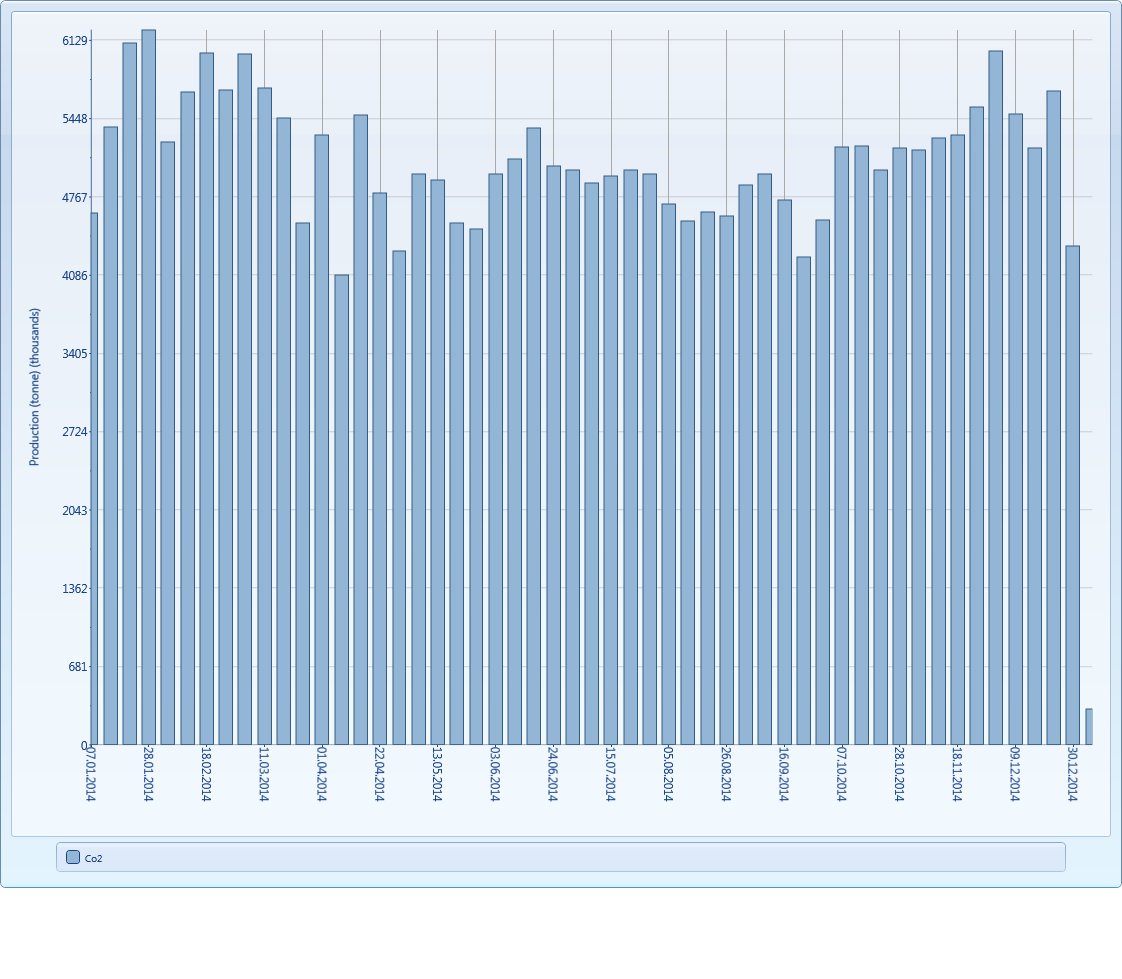
\includegraphics[width=13cm,keepaspectratio=true]{figures/MTCO2}
\caption{Total emissions for normal inflow 2014}
\label{fig:MTemissionsnormal}
\end{center}
\end{figure}
\paragraph{Price\\}
Energy prices for the different weeks of 2014 for the analyzed countries are shown in figure \ref{fig:MTpricesnormal}. In this graph it can be obtained that prices in Norway are the lowest because of the high amount of renewable energy. The energy prices in Germany are the highest because of some coal and gas power. Generally the prices during the summer are lower than in the heating season. This is because in summer there is less need for energy due to non-running heating systems.
\begin{figure}[htbp]
\begin{center}
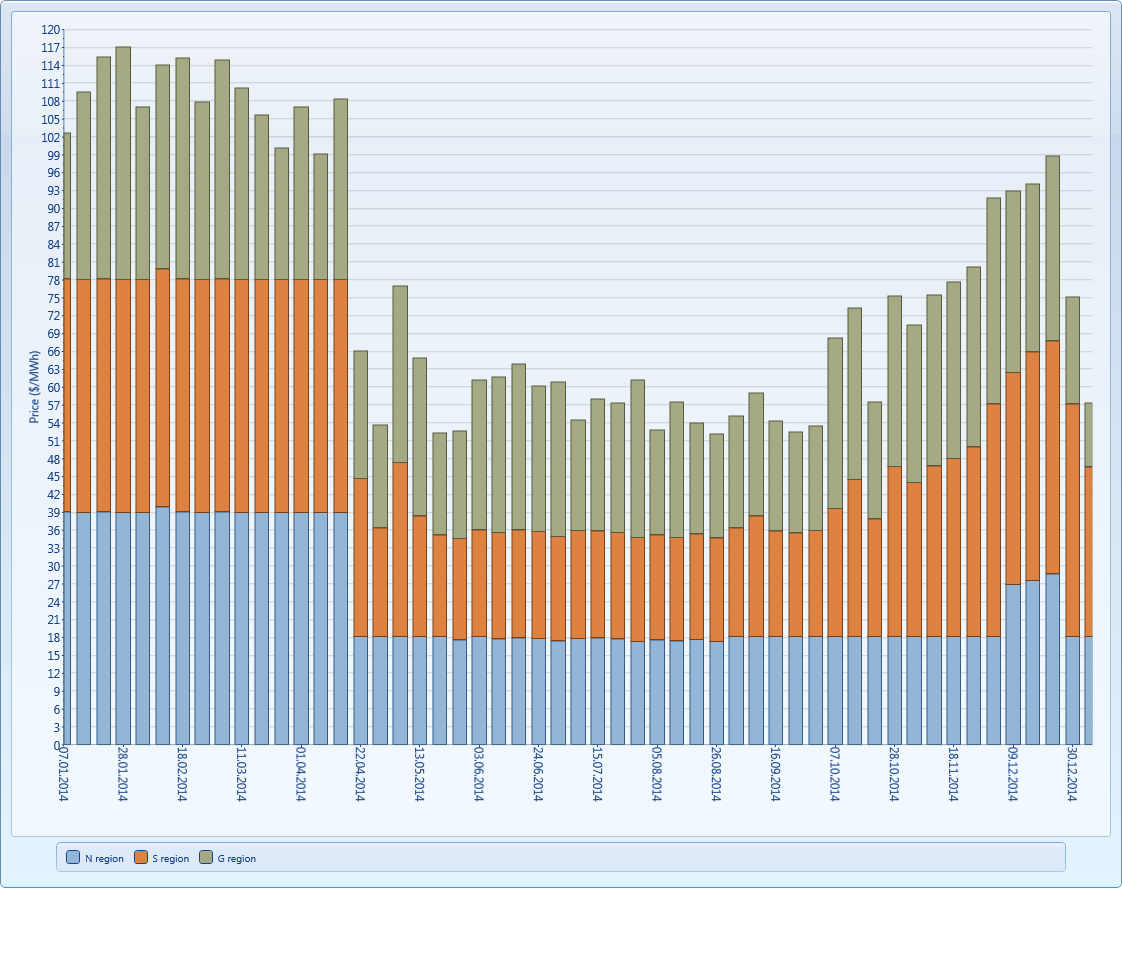
\includegraphics[width=13cm,keepaspectratio=true]{figures/MTprices}
\caption{Calculcated prices with normal inflow}
\label{fig:MTpricesnormal}
\end{center}
\end{figure}

%-------------------------------------------------------------------------------
% low inflow scenario
%-------------------------------------------------------------------------------
\subsubsection{Low inflow scenario}
In this scenario a dry year with an inflow below the average was assumed. 
\paragraph{Optimal generation dispatch\\}
The optimal generation dispatch can be found in Appendix \ref{apx:figures} in figure \ref{fig:MTgenerationGdry} (Germany), figure \ref{fig:MTgenerationSdry} (Sweden) as well as figure \ref{fig:MTgenerationNdry} (Norway).
\begin{itemize}
\item Germany\\
Due to the fact that there is no renewable energy in Germany, the simulated results remain mostly the same. 
\item Sweden\\
Because of lower inflow the amount of energy produced with small hydro is lower than in average case. More energy is produced with reservoir hydro, but in dry years the production is a little bit lower than in the average simulation case.
\item Norway\\
Also in Norway the overall production decreases in the dry case. It can be obtained that during the heating season the difference to the average inflow is not significant. Most power is produced with reservoir hydro units. In summer the production is mainly done with small hydro power, which is quite different to the average. In dry years some gas production is used during the whole period.
\end{itemize}

\paragraph{Transmission\\}
The power transmission on the powerlines between Norway, Sweden and Germany can be found in Appendix \ref{apx:figures} in  figure \ref{fig:MTnodetransmissiondry}. In the dry inflow case it can be seen that the flow between Germany and Norway is almost constant over the whole year. Between Sweden and Germany is hardly any flow, while the energy transmission in summer increases very much.

\paragraph{Emission\\}
$CO_2$-emissions for the whole year 2014 are shown in Appendix \ref{apx:figures} in figure \ref{fig:MTemissionsdry}. Compared to the average inflow scenario the emissions in Norway are a little bit higher. This is because more power is produced with the gas generation unit. The most emissions are generated in Germany.

\paragraph{Price\\}
The energy prices for a dry year 2014 are plotted in Appendix \ref{apx:figures} in figure \ref{fig:MTpriceslow}. Compared to the average inflow simulation, the prices are more constant over the year. The price level is higher due to lower renewable power production.

%-------------------------------------------------------------------------------
% high inflow scenario
%-------------------------------------------------------------------------------
\subsubsection{High inflow scenario}
This scenario uses a very wet year 2014. 
\paragraph{Optimal generation dispatch\\}
Optimal generation for Sweden is shown in Appendix \ref{apx:figures} in figure \ref{fig:MTgenerationSwet}. The generation dispatch for Norway can be seen in figure \ref{fig:MTgenerationNwet}, the german production in figure \ref{fig:MTgenerationGwet}.
\begin{itemize}
\item Germany\\
As in the average in the average inflow scenario and the low inflow scenario, the generation dispatch in Germany does not change significant due to the fact that no renewable power is installed.
\item Sweden\\
With high inflow the base load is also covered with nuclear and coal power. It can be obtained that mostly all peak power is produced with renewable generation units. During the heating season the peak power is produced with reservoir hydro power, in summer most peak power is produced with small hydro generation. Some additional power is produced with wind power during whole year, oil and gas generation is hardly used.
\item Norway\\
All power is produced by renewables in the high inflow scenario. The generation dispatch is like the dispatch in the average scenario, but more power is produced.
\end{itemize}

\paragraph{Transmission\\}
The usage of the transmission lines between Sweden, Norway and Germany for high inflow into reservoirs is shown in Appendix \ref{apx:figures} in figure \ref{fig:MTnodetransmissionwet}. During heating season there is only transmission between Sweden and Germany, in the summer months there are huge transmissions between Sweden, Norway and Germany. Over the whole year there is very small transmissions between Germany and Norway.

\paragraph{Emission\\}
Emissions of carbon dioxide by running thermal power plants for this scenario are plotted in Appendix \ref{apx:figures} in figure \ref{fig:MTemissionswet}. Due to the effect that Germany produces only non-renewable power the emissions decrease not very much in the high inflow scenario. They are a little bit smaller, so it can be said that some energy is transferred from renewable energy to Germany. 

\paragraph{price\\}
The energy prices for a whole year 2014 with high inflow is shown in Appendix \ref{apx:figures} in figure \ref{fig:MTpriceswet}. The prices in Sweden are stable over whole the year, in Norway they are a little bit higher during the heating season. Over all the prices are lower the more inflow to the reservoirs is.

%-------------------------------------------------------------------------------
% expansion planning
%-------------------------------------------------------------------------------
\subsection{Expansion planning}
The need of energy changes over time. It is important to simulate future trends in energy production to find the optimal object, size and time. In this model the situation is expected to change over the next 20 years. Fuel prices are expected to increase for all types of fuels except lignite, uranium and bio fuel. The demand for electricity is expected to decrease in Continental Europe represented by Germany, stays stable in Sweden and increase in Norway. The three countries want to reduce $CO_2$ Emissions with an approach to stimulate increased investments in renewable energy sources. The simulation is done with two different approaches and a combined version.
\begin{itemize}
\item green certificates\\
To push investments in new renewables, producers of new wind, solar and small hydro plants are awarded with 50 NOK/kWh. This incentive leads to the fact that new wind power plants and also new small hydro power plants get profitable and therefore built as you can see in Figure \ref{fig:CapacityBuiltNewGenGC}. For solar power plant the subsidy is still too low to get profitable due to the high investment costs. Figure \ref{fig:CapacityBuiltNewGenGC} show nicely that investments will be mainly made in the Nordic Countries where you have a great potential for wind and hydro energy. Sweden and Norway will invest in the beginning of the expansion planning. This shows that the set subsidy has an impact on the producers. Germany is not affected by this impact and will invest at the end of the expansion period in a new nuclear power plant. Figure \ref{fig:BuildCostGC} points out that especially the built costs for the wind power plants are quite low while the costs for building the nuclear power plant are a lot higher. The green certificate approach reduces CO2 emissions as desired (Figure \ref{fig:Co2ProductionGC}). The emissions are reduced more or less steadily from the beginning on.
\item emission tax\\
The Emission tax approach does not award producers who invest in renewables. In order to make renewables more competitive a tax on $CO_2$ is set to 0.05 NOK/kg.  The Emission tax approach has a similar effect as the green certificate approach and leads to increasing investments in the beginning of the expansion period. Figure \ref{fig:CapacityBuiltNewGenET} in Appendix \ref{apx:figures} reveals that compared to the green certificate case the investments here are not just made on renewables. Germany invests in a new nuclear plant in the beginning of the expansion. Nuclear power plants produce a low amount of $CO_2$ and benefits as well from the set tax. Norway will invest a lot in new small hydro plants and a bit in wind. Wind power plants are not as competitive as in the green certificate approach.\\
At the end of the simulation period Germany will invest in a new gas power plant. The built cost for the new gas plant are quite low (figure \ref{fig:BuildCostET}). The emission tax is not working as desired in this case. Figure \ref{fig:Co2ProductionET} show that the $CO_2$ emissions sink in the beginning when Norway builds new hydro capacities and Germany invests in nuclear. But then there is no further reduction and the emission level is even rising at the end due to the new built gas capacities.
\end{itemize}
As planning horizon a period of 20 years was taken, which is quite common for expansion planning simulations. For a better understanding of the two approaches the simulation is also made for just the retirement plan without further incentives for the renewables. Figure \ref{fig:capacitywithout}in Appendix  \ref{apx:figures} shows that renewables such as wind and solar are not competitive enough without further help.  Norway will invest in a new small hydro plants and Germany in nuclear. Both of them will make the investment after some years because they don´t have further incentives to invest earlier. Figure \ref{fig:CO2without} points out that the $CO_2$ emissions are decreasing over the simulation period even with no further help for renewables. Since both Norway and Germany will invest in new plants with a low production of $CO_2$. The reduction is however slower than with the extra stimulation.
%\begin{figure}[htbp]
%\begin{center}
%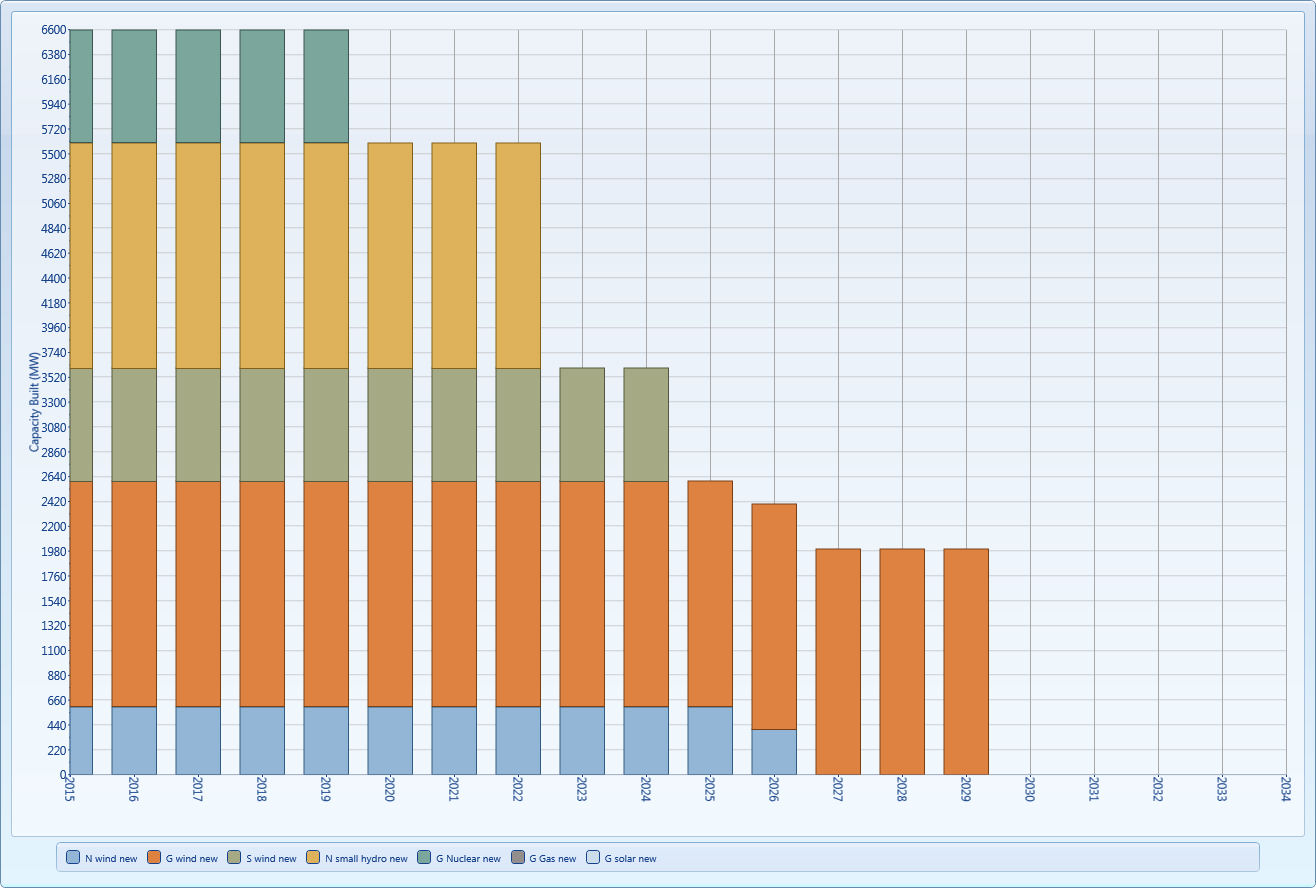
\includegraphics[width=13cm,keepaspectratio=true]{figures/Expansion/CapacityBuiltETGC}
%\caption{}
%\label{fig:CapacityBuiltETGC}
%\end{center}
%\end{figure}
%\begin{figure}[htbp]
%\begin{center}
%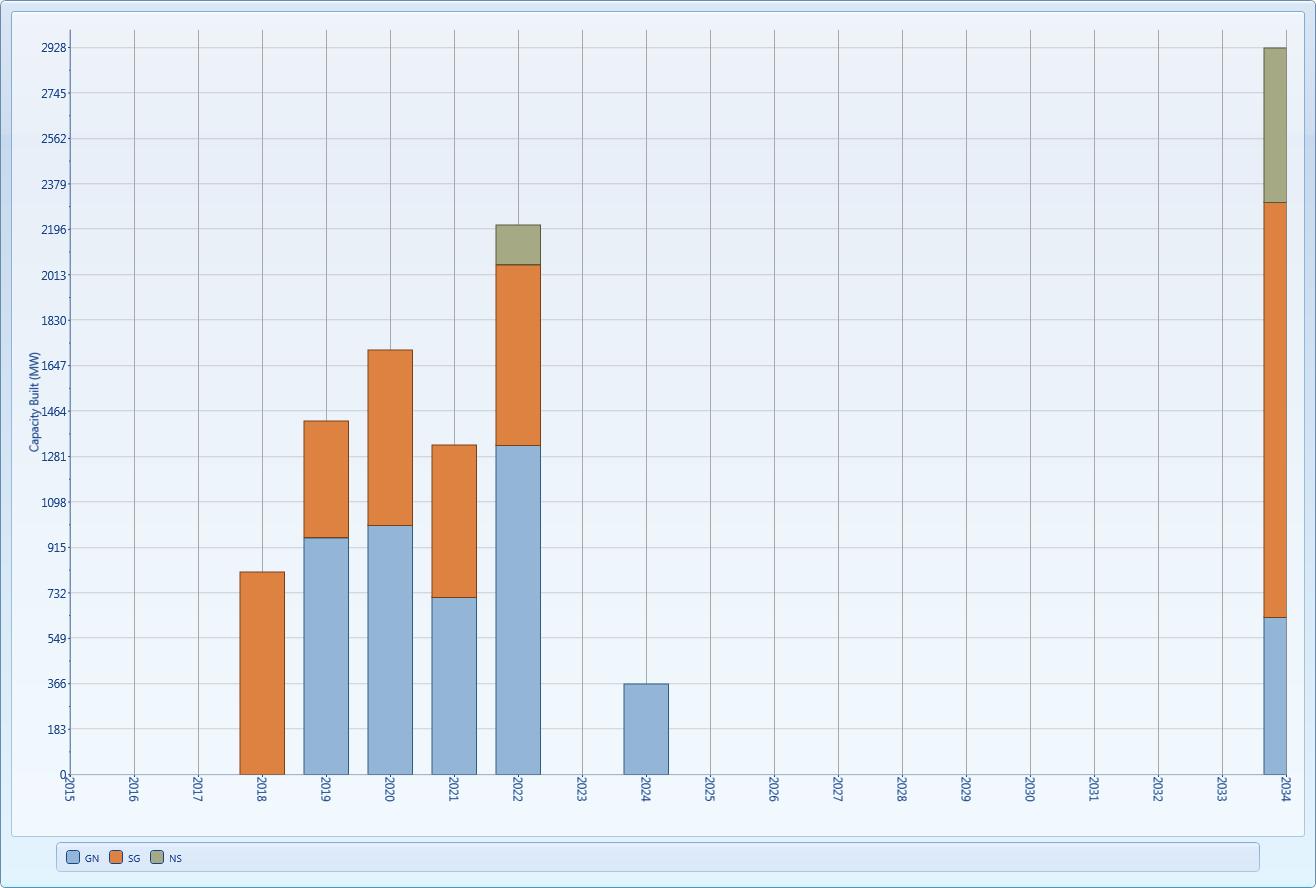
\includegraphics[width=13cm,keepaspectratio=true]{figures/Expansion/CapacityBuiltInterfacesETGC}
%\caption{}
%\label{fig:CapacityBuiltInterfacesETGC}
%\end{center}
%\end{figure}
%\begin{figure}[htbp]
%\begin{center}
%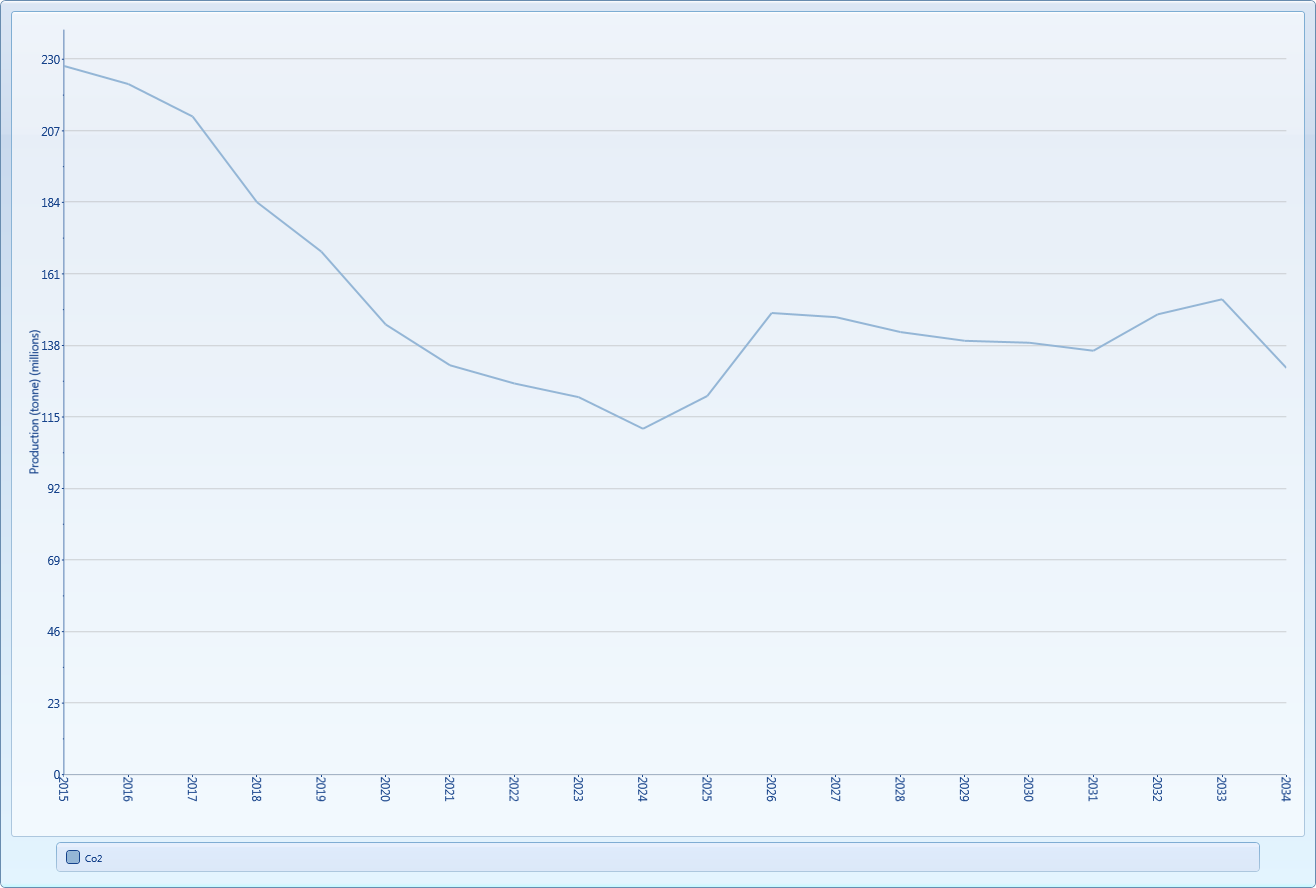
\includegraphics[width=13cm,keepaspectratio=true]{figures/Expansion/Co2ProductionETGC}
%\caption{}
%\label{fig:Co2ProductionETGC}
%\end{center}
%\end{figure}
\begin{figure}[htbp]
\begin{center}
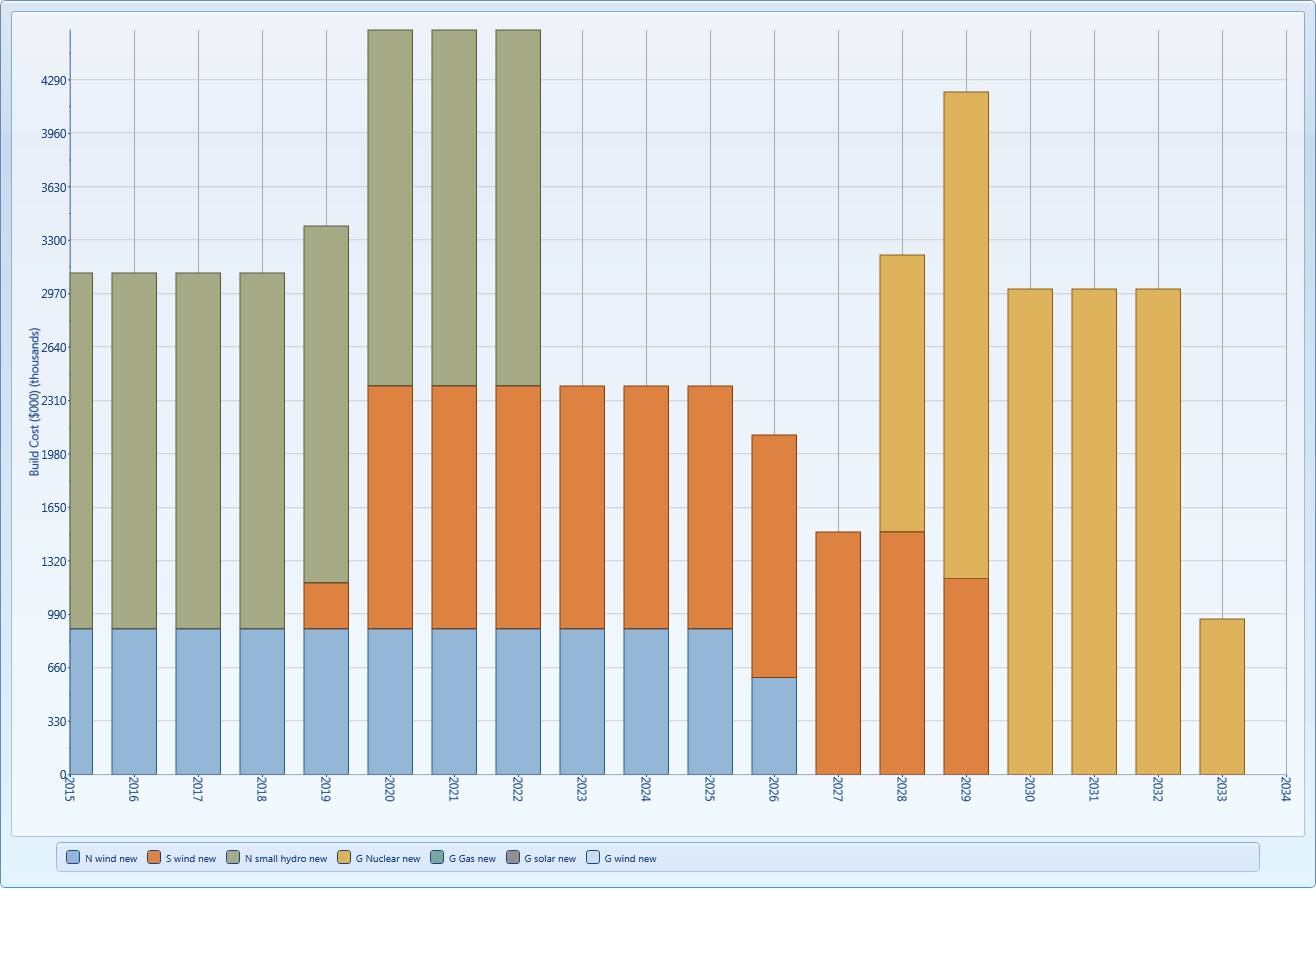
\includegraphics[width=13cm,keepaspectratio=true]{figures/Expansion/GreenCertificate/BuildCostGC}
\caption{Build costs using the green certificate support scheme}
\label{fig:BuildCostGC}
\end{center}
\end{figure}
\begin{figure}[htbp]
\begin{center}
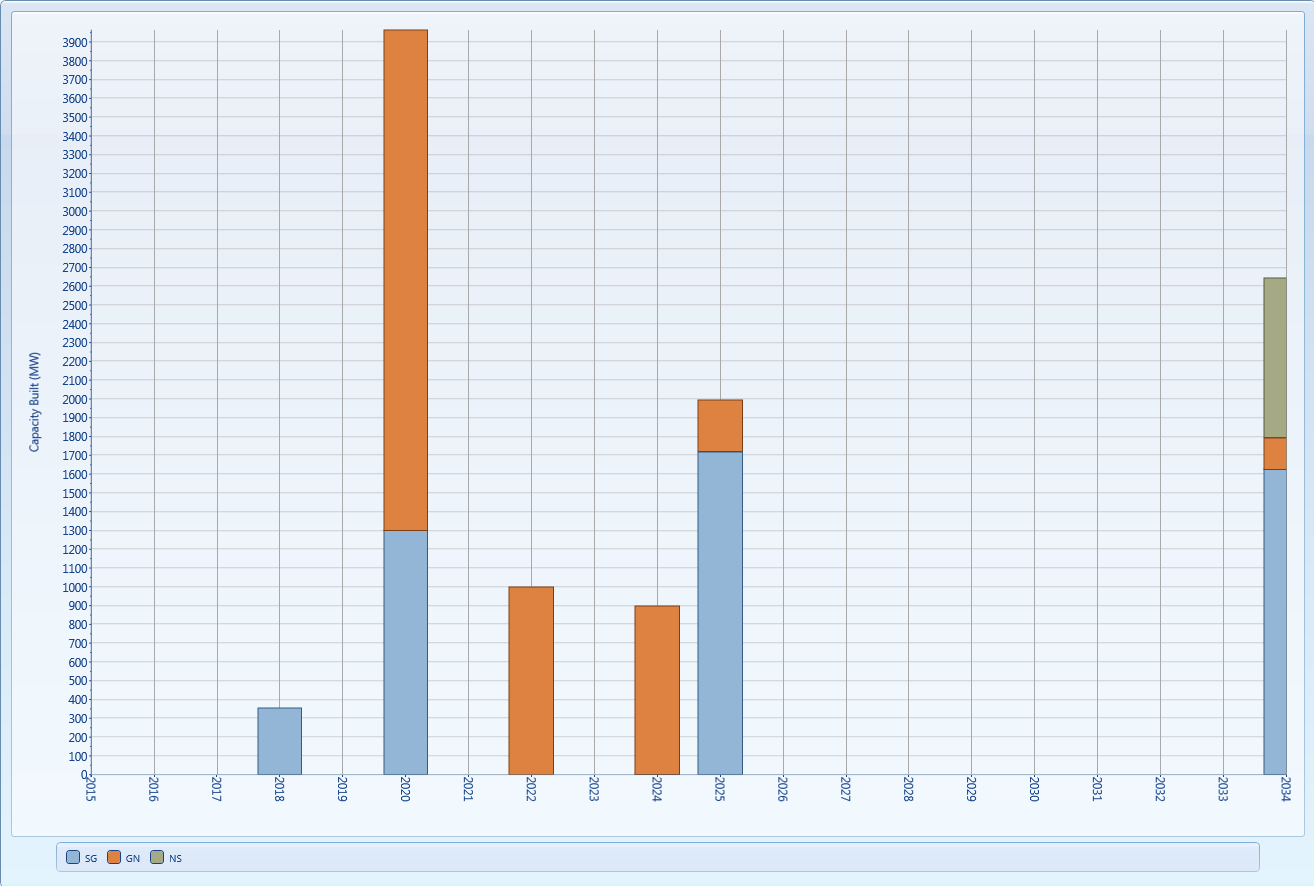
\includegraphics[width=13cm,keepaspectratio=true]{figures/Expansion/GreenCertificate/CapacityBuiltInterfaceGC}
\caption{Built interface sizes with green certificates}
\label{fig:CapacityBuiltInterfaceGC}
\end{center}
\end{figure}
\begin{figure}[htbp]
\begin{center}
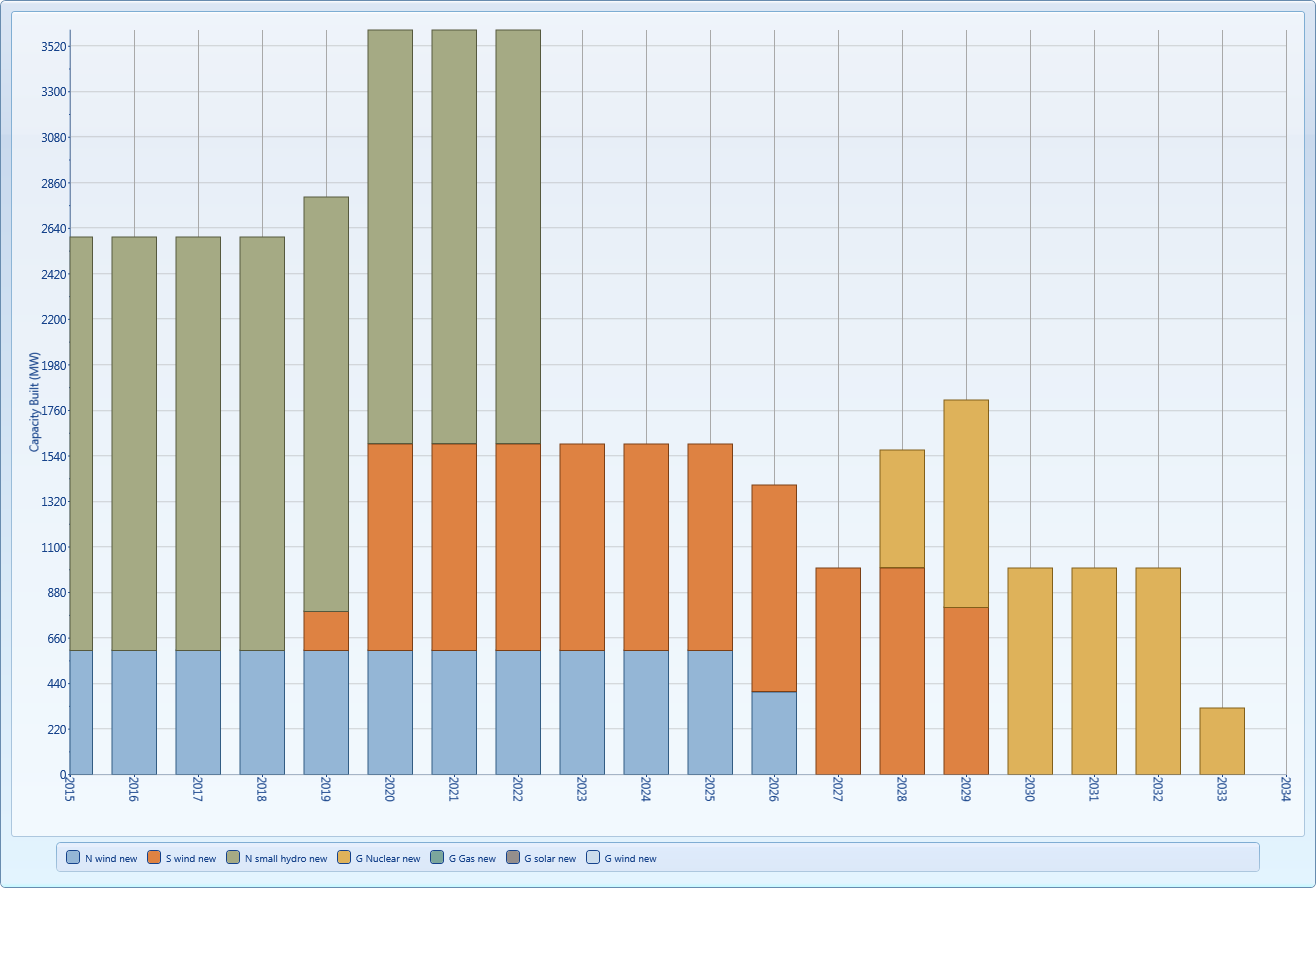
\includegraphics[width=13cm,keepaspectratio=true]{figures/Expansion/GreenCertificate/CapacityBuiltNewGenGC}
\caption{New capacities built using green certificates}
\label{fig:CapacityBuiltNewGenGC}
\end{center}
\end{figure}
\begin{figure}[htbp]
\begin{center}
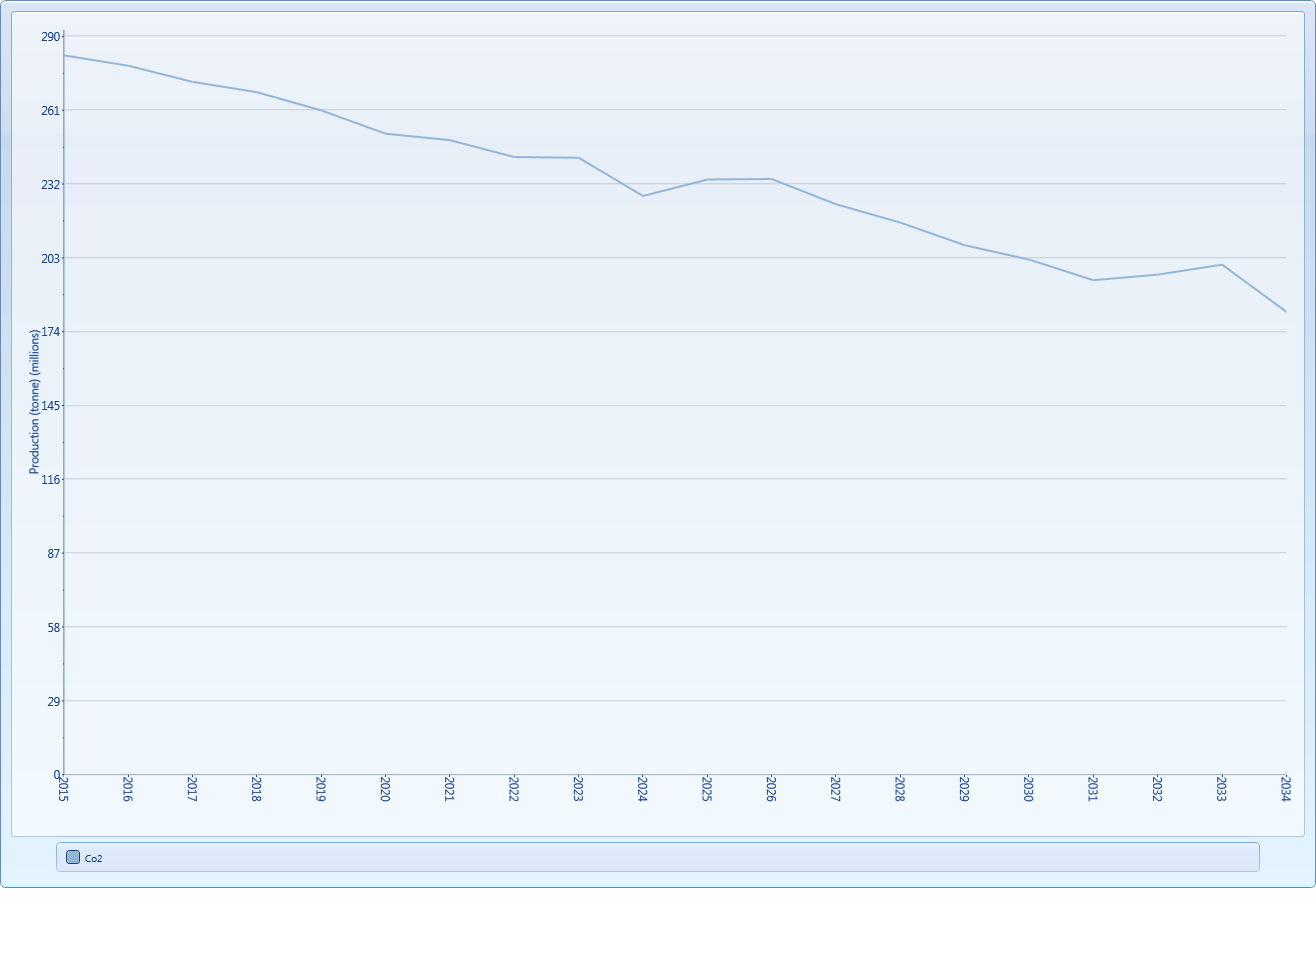
\includegraphics[width=13cm,keepaspectratio=true]{figures/Expansion/GreenCertificate/Co2ProductionGC}
\caption{development of $CO_2$-emissions when support with green certificates}
\label{fig:Co2ProductionGC}
\end{center}
\end{figure}



\newpage
\section{Conclusion}


%-------------------------------------------------------------------------------
%-------------------------------------------------------------------------------
% APPENDIX
%-------------------------------------------------------------------------------
%-------------------------------------------------------------------------------

\newpage
\appendix
\section{Additional Figures\label{apx:figures}}
%-------------------------------------------------------------------------------
% low inflow scenario
%-------------------------------------------------------------------------------
\begin{figure}[htbp]
\begin{center}
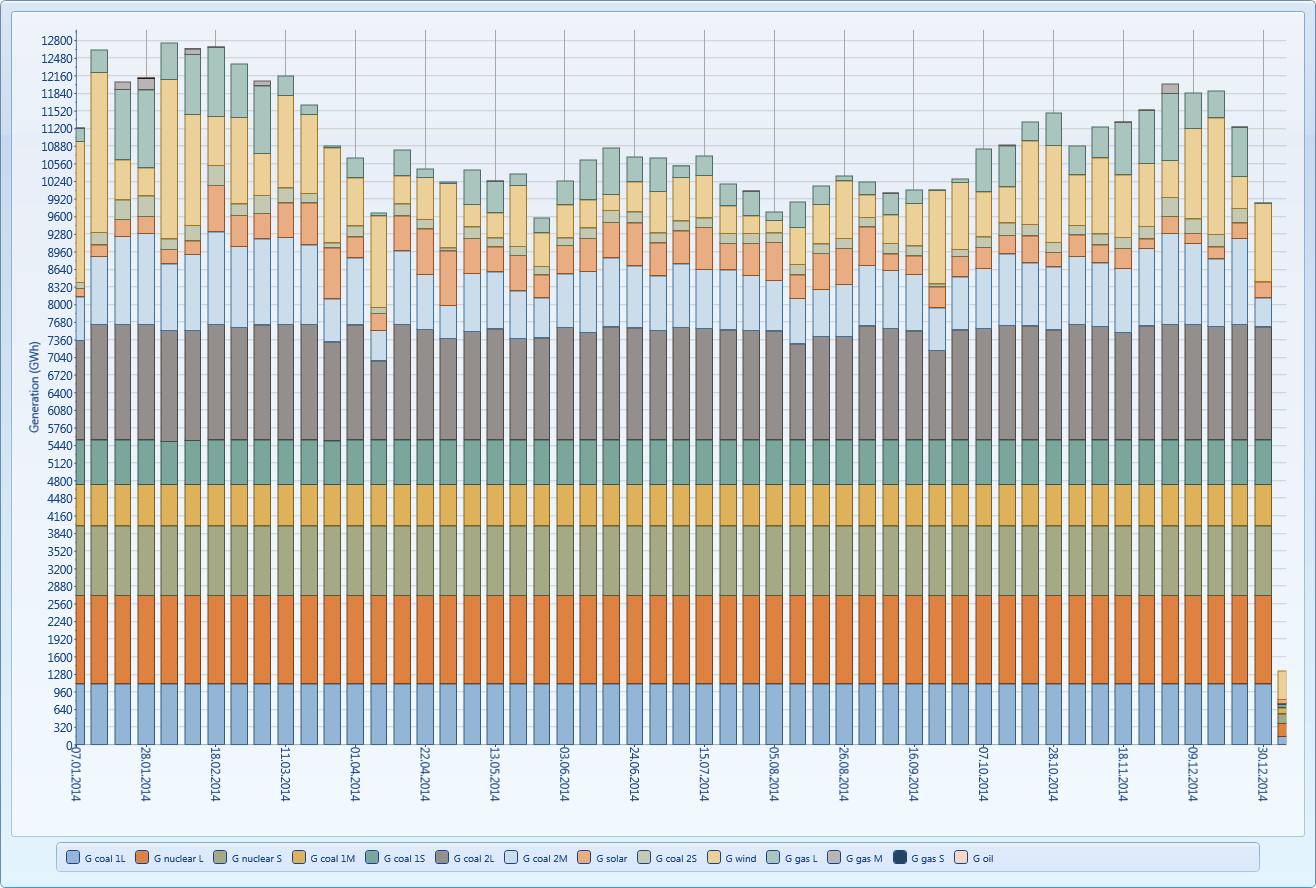
\includegraphics[width=13cm,keepaspectratio=true]{figures/drycase/MTgenerationGdry}
\caption{Optimal generation dispatch for Germany 2014 with low inflow}
\label{fig:MTgenerationGdry}
\end{center}
\end{figure}
\begin{figure}[htbp]
\begin{center}
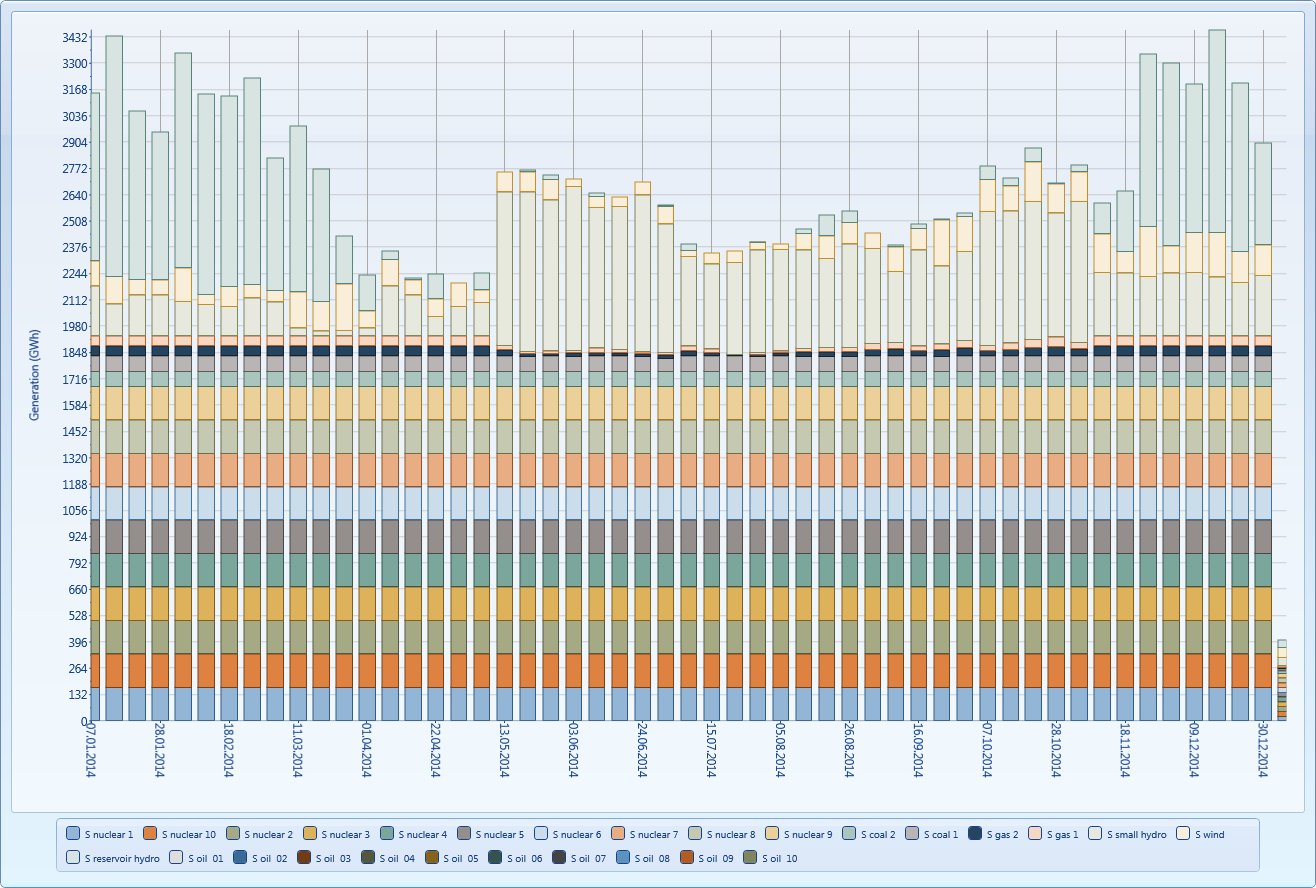
\includegraphics[width=13cm,keepaspectratio=true]{figures/drycase/MTgenerationSdry}
\caption{Optimal generation dispatch for Sweden 2014 with low inflow}
\label{fig:MTgenerationSdry}
\end{center}
\end{figure}
\begin{figure}[htbp]
\begin{center}
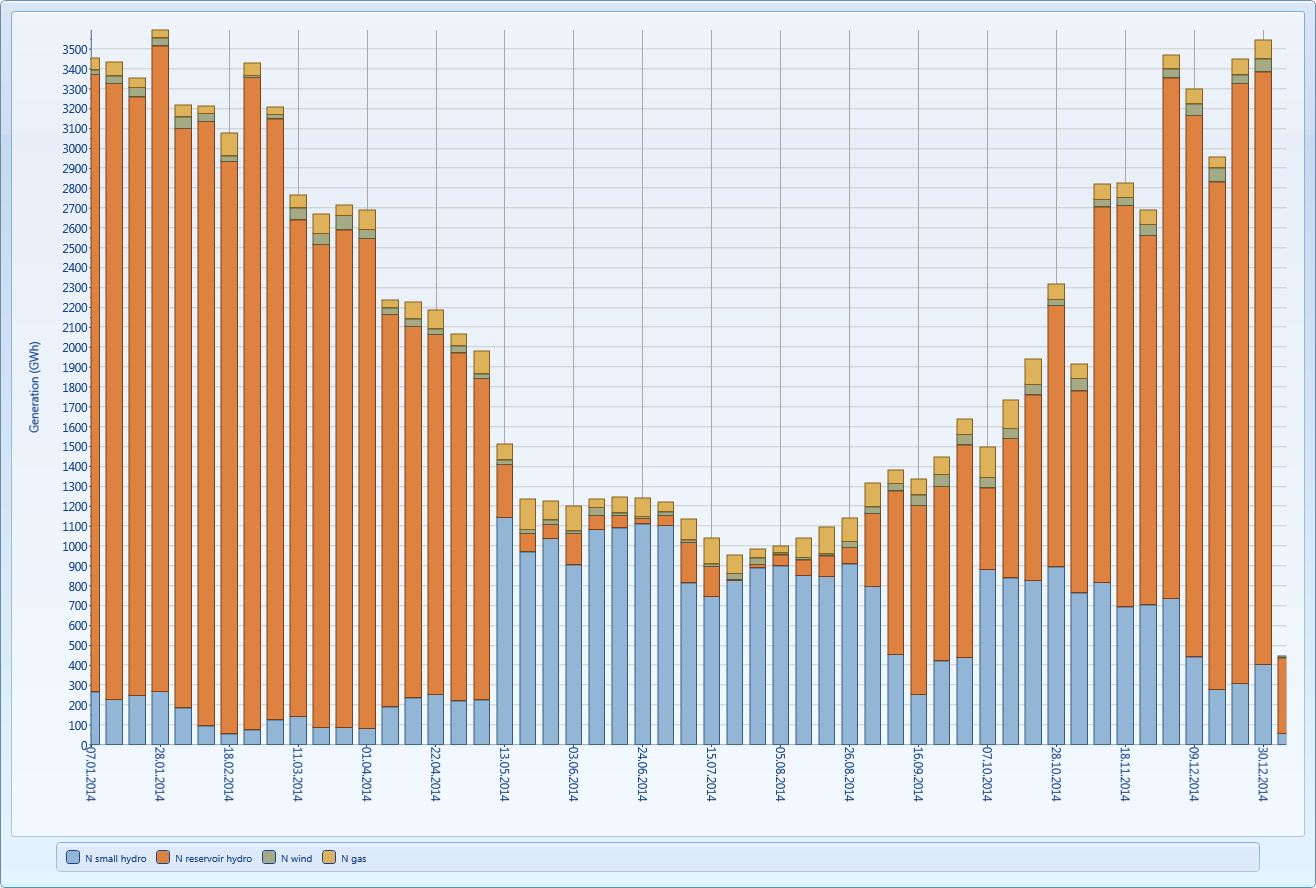
\includegraphics[width=13cm,keepaspectratio=true]{figures/drycase/MTgenerationNdry}
\caption{Optimal generation dispatch for Norway 2014 with low inflow}
\label{fig:MTgenerationNdry}
\end{center}
\end{figure}
\begin{figure}[htbp]
\begin{center}
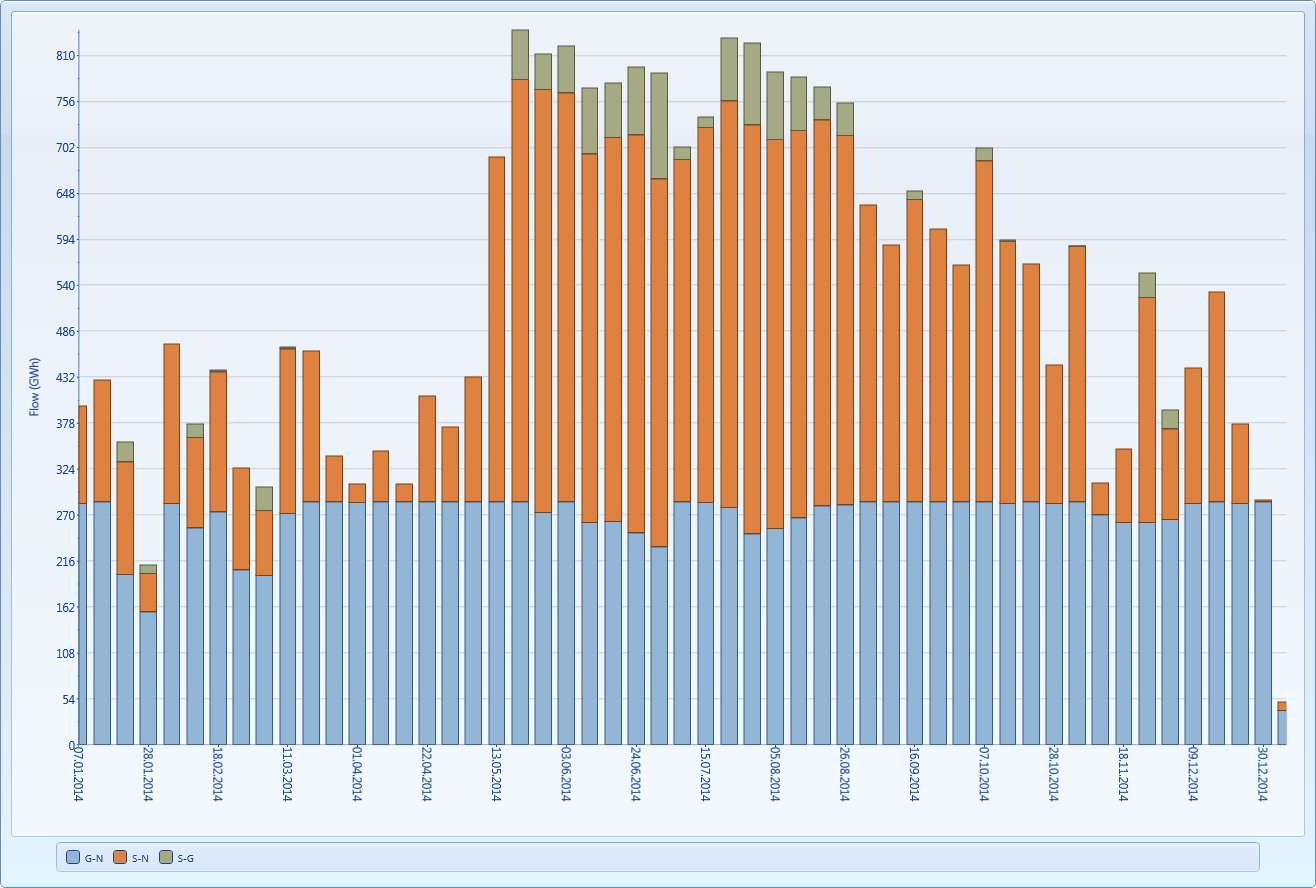
\includegraphics[width=13cm,keepaspectratio=true]{figures/drycase/MTnodetransmissiondry}
\caption{Transmission between N/W/S with low inflow}
\label{fig:MTnodetransmissiondry}
\end{center}
\end{figure}
\begin{figure}[htbp]
\begin{center}
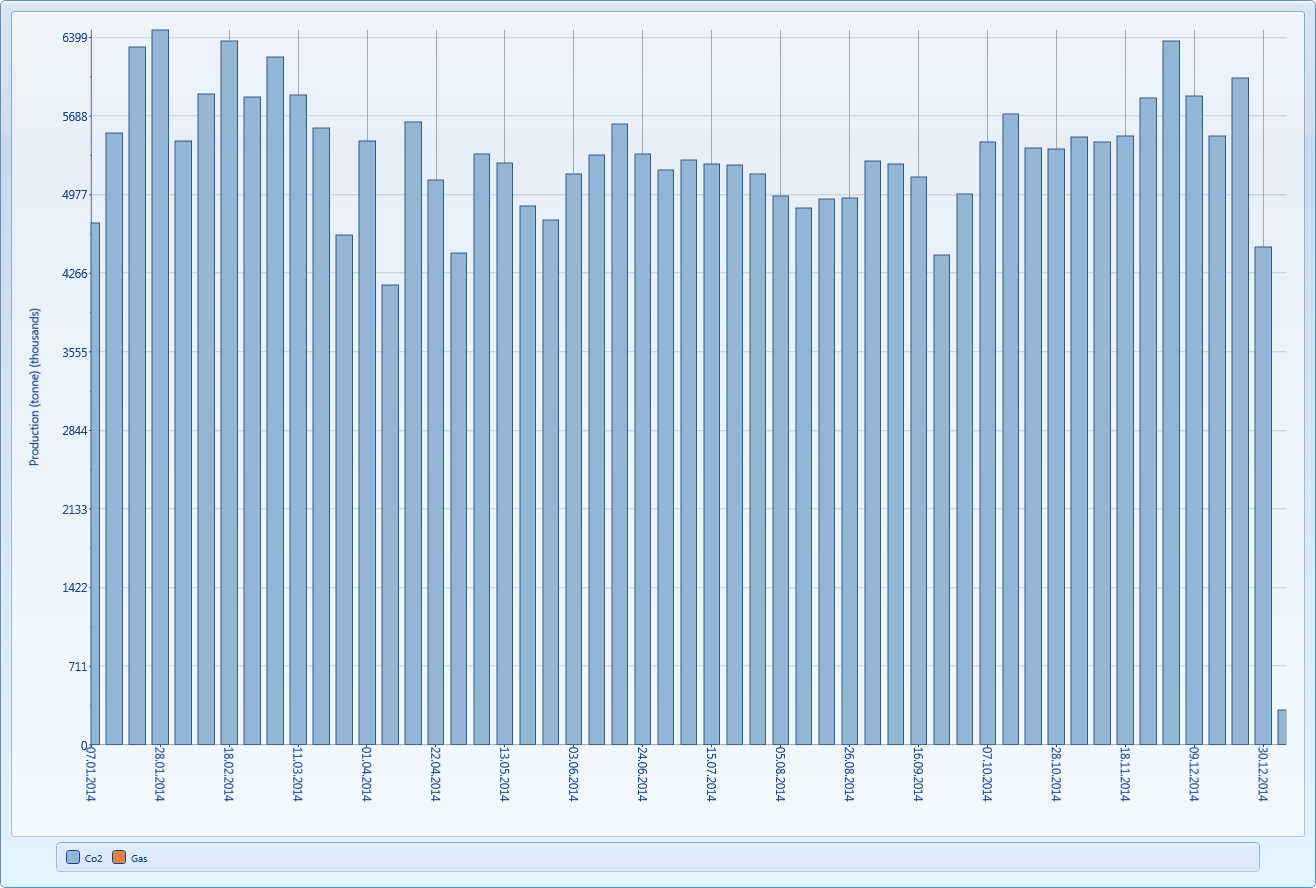
\includegraphics[width=13cm,keepaspectratio=true]{figures/drycase/MTCO2dry}
\caption{Total $CO_2$-emissions for low inflow 2014}
\label{fig:MTemissionsdry}
\end{center}
\end{figure}
\begin{figure}[htbp]
\begin{center}
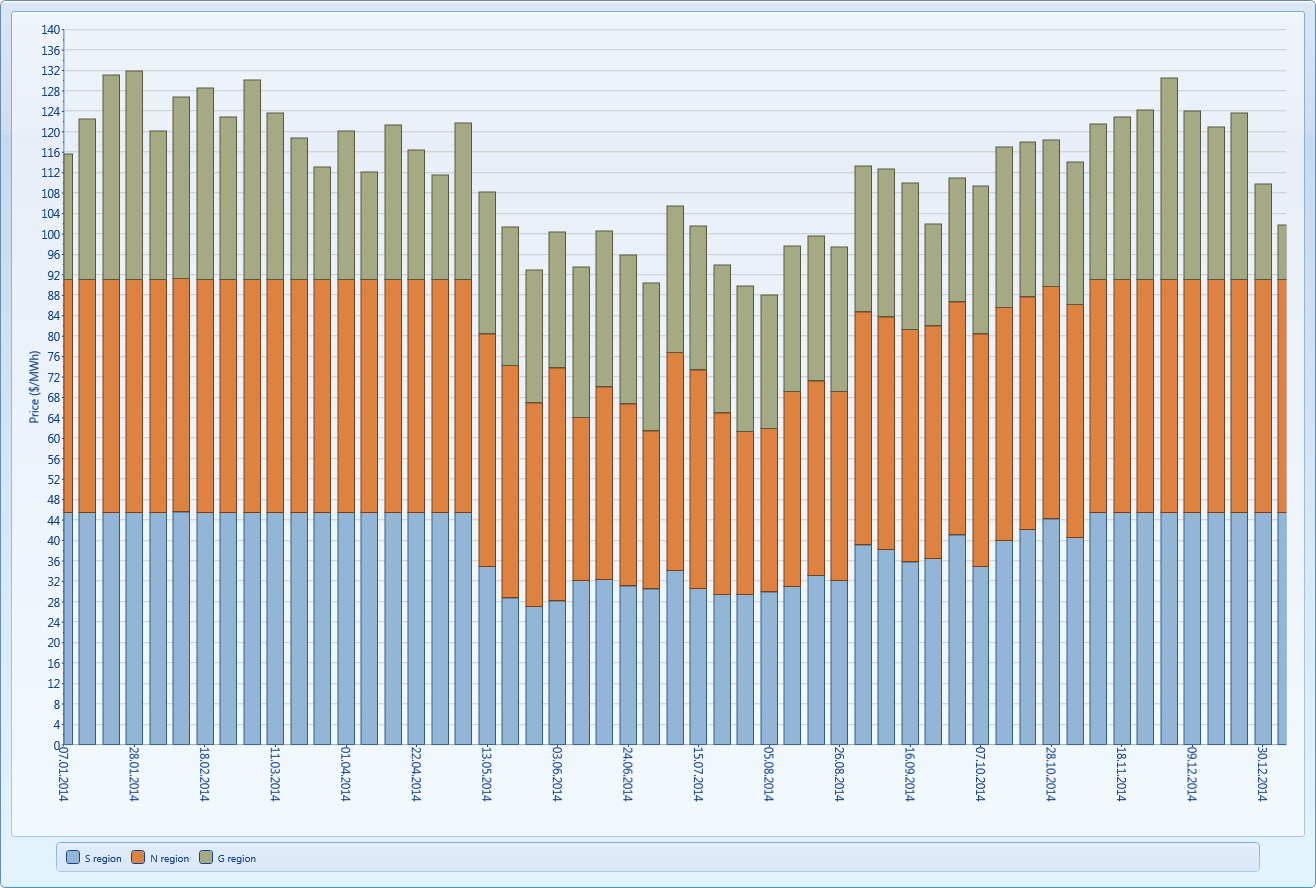
\includegraphics[width=13cm,keepaspectratio=true]{figures/drycase/MTpricesdry}
\caption{Calculcated prices with low inflow}
\label{fig:MTpriceslow}
\end{center}
\end{figure}
%-------------------------------------------------------------------------------
% high inflow scenario
%-------------------------------------------------------------------------------
\begin{figure}[htbp]
\begin{center}
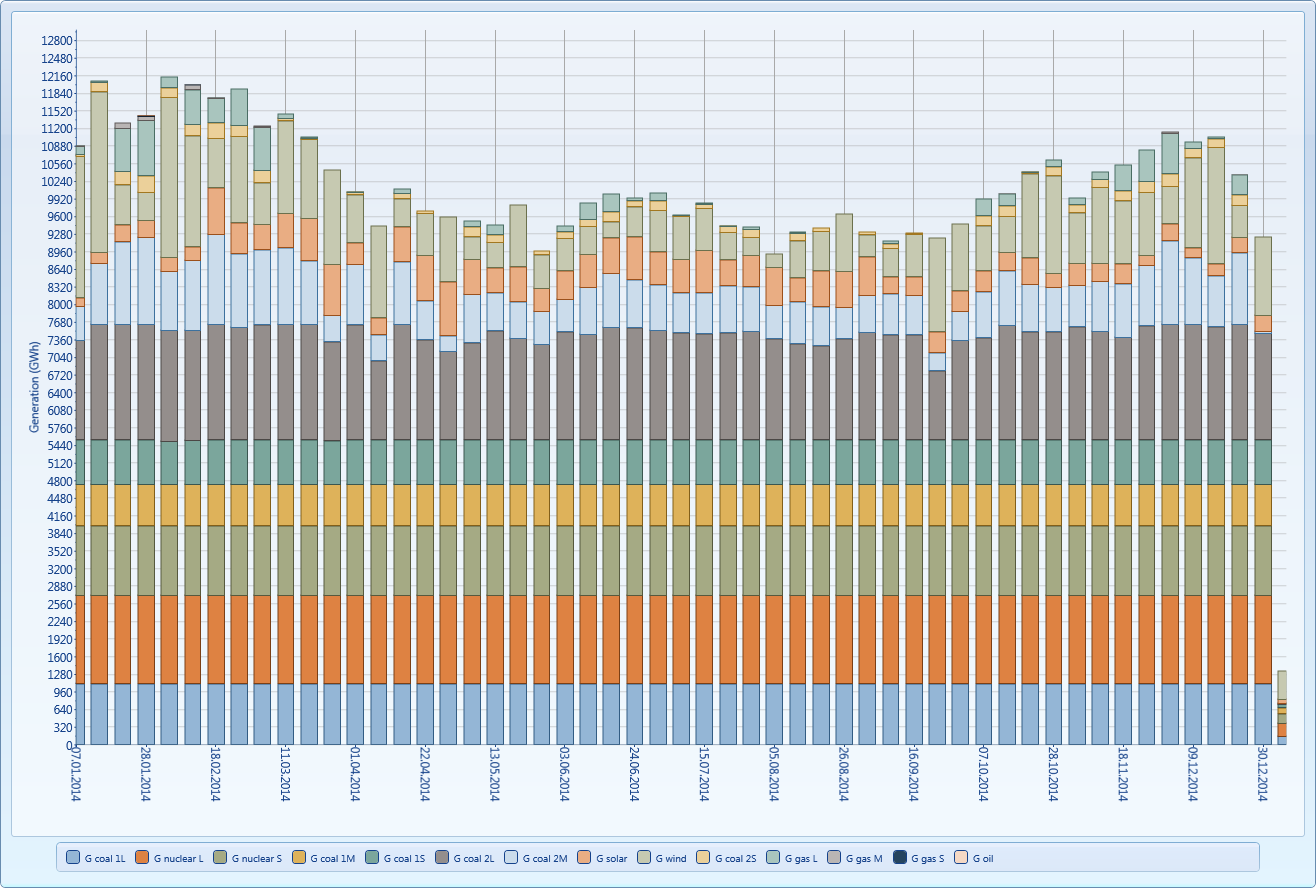
\includegraphics[width=13cm,keepaspectratio=true]{figures/wetcase/MTgenerationGwet}
\caption{Optimal generation dispatch for Germany 2014 with high inflow}
\label{fig:MTgenerationGwet}
\end{center}
\end{figure}
\begin{figure}[htbp]
\begin{center}
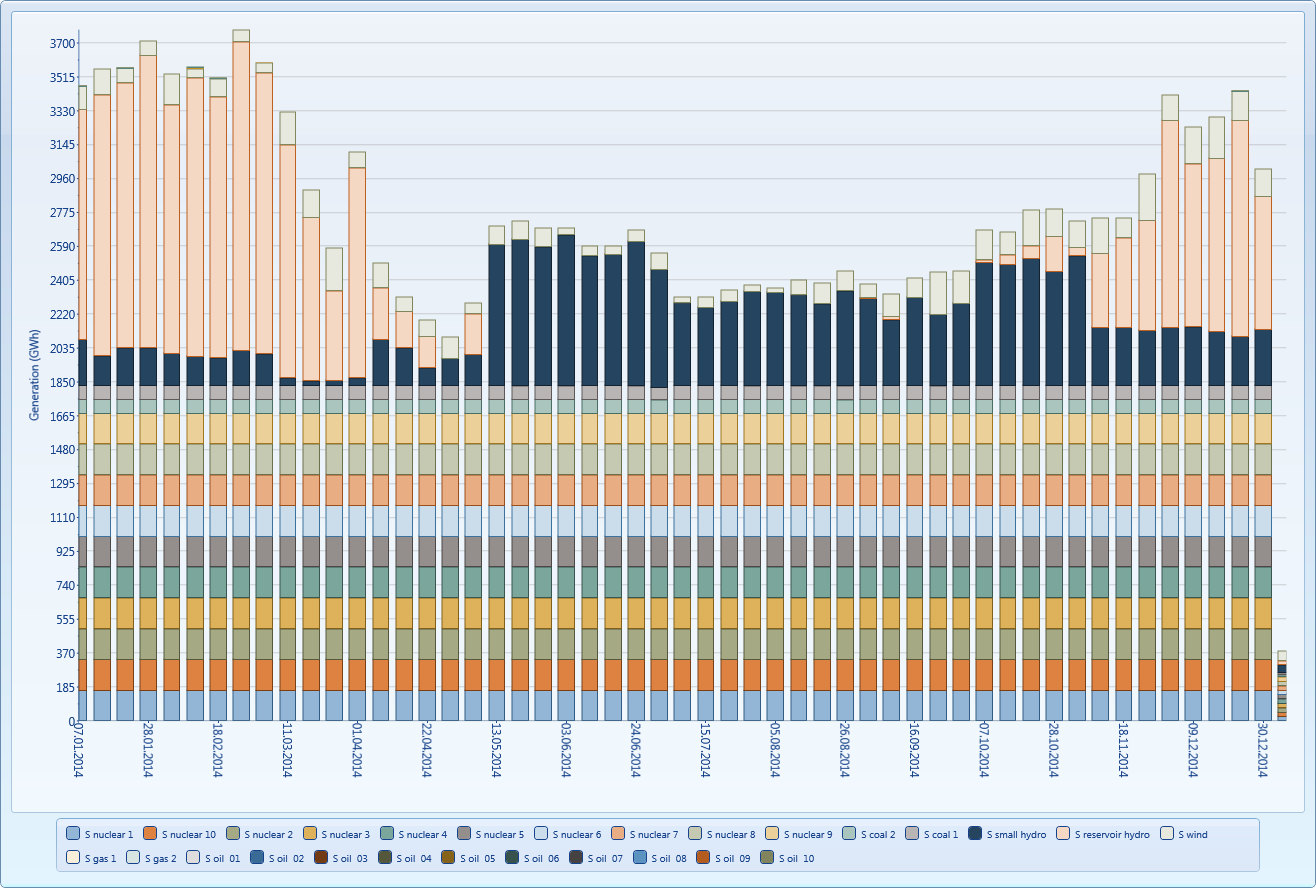
\includegraphics[width=13cm,keepaspectratio=true]{figures/wetcase/MTgenerationSwet}
\caption{Optimal generation dispatch for Sweden 2014 with high inflow}
\label{fig:MTgenerationSwet}
\end{center}
\end{figure}
\begin{figure}[htbp]
\begin{center}
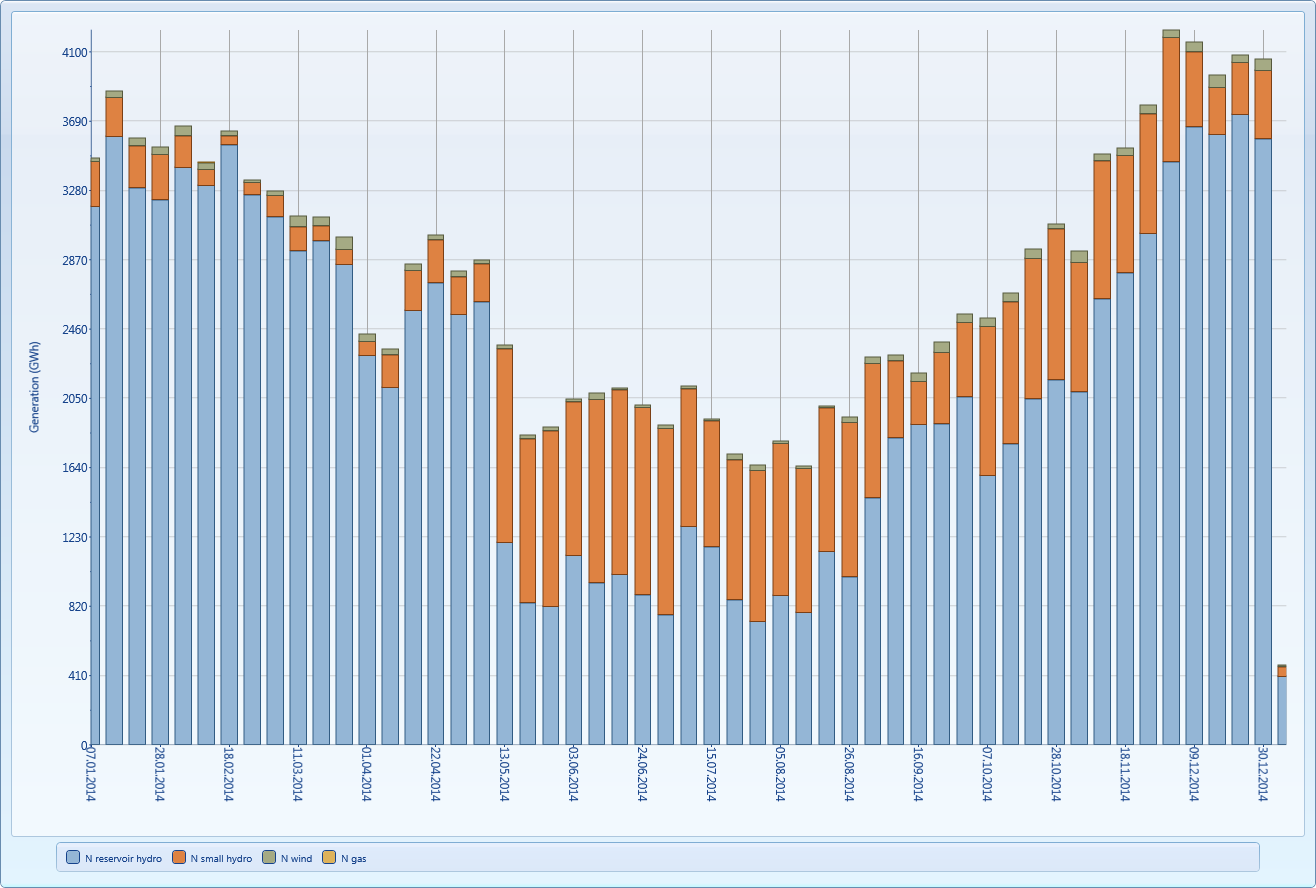
\includegraphics[width=13cm,keepaspectratio=true]{figures/wetcase/MTgenerationNwet}
\caption{Optimal generation dispatch for Norway 2014 with high inflow}
\label{fig:MTgenerationNwet}
\end{center}
\end{figure}
\begin{figure}[htbp]
\begin{center}
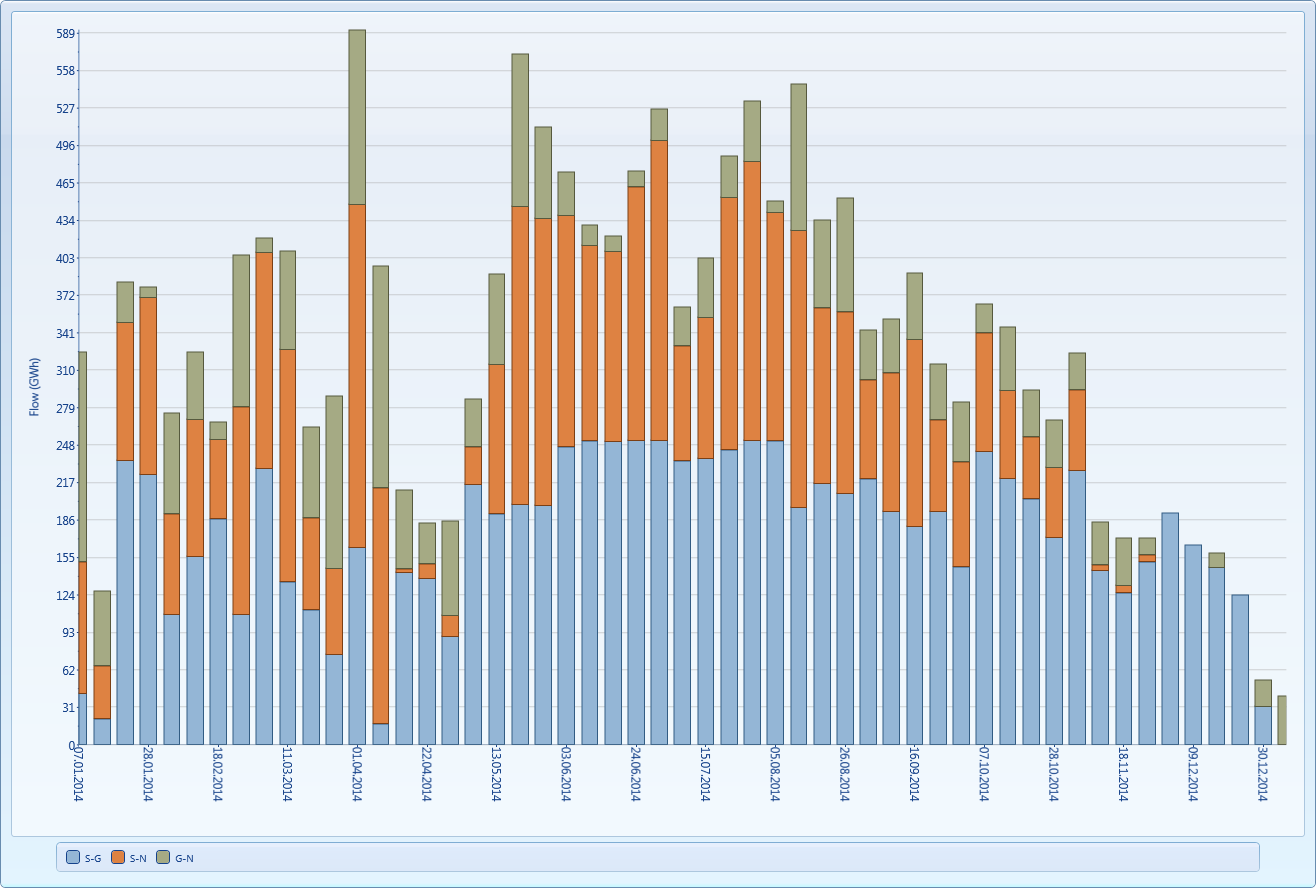
\includegraphics[width=13cm,keepaspectratio=true]{figures/wetcase/MTnodetransmissionwet}
\caption{Transmission between N/W/S with high inflow}
\label{fig:MTnodetransmissionwet}
\end{center}
\end{figure}
\begin{figure}[htbp]
\begin{center}
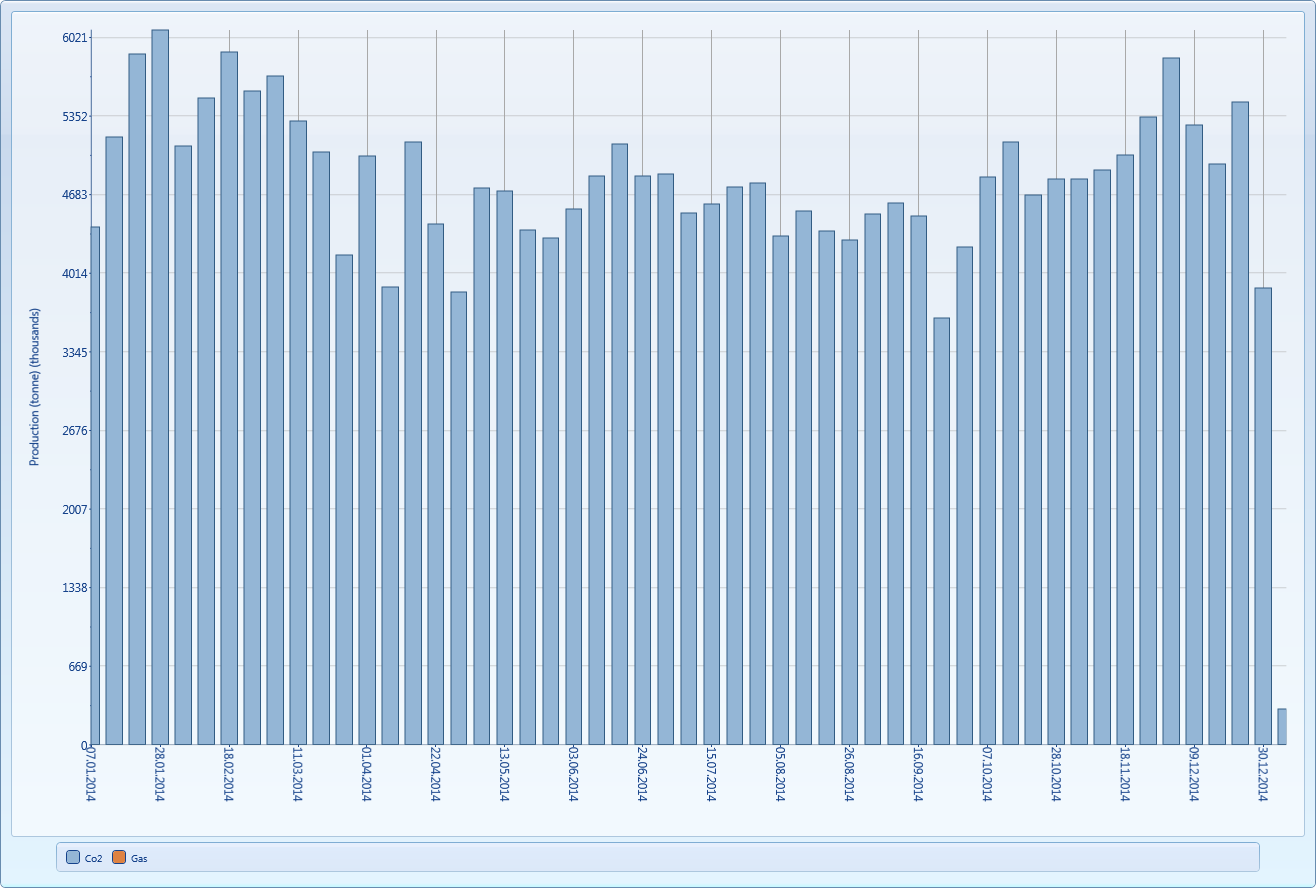
\includegraphics[width=13cm,keepaspectratio=true]{figures/wetcase/MTCO2wet}
\caption{Total $CO_2$-emissions for high inflow 2014}
\label{fig:MTemissionswet}
\end{center}
\end{figure}
\begin{figure}[htbp]
\begin{center}
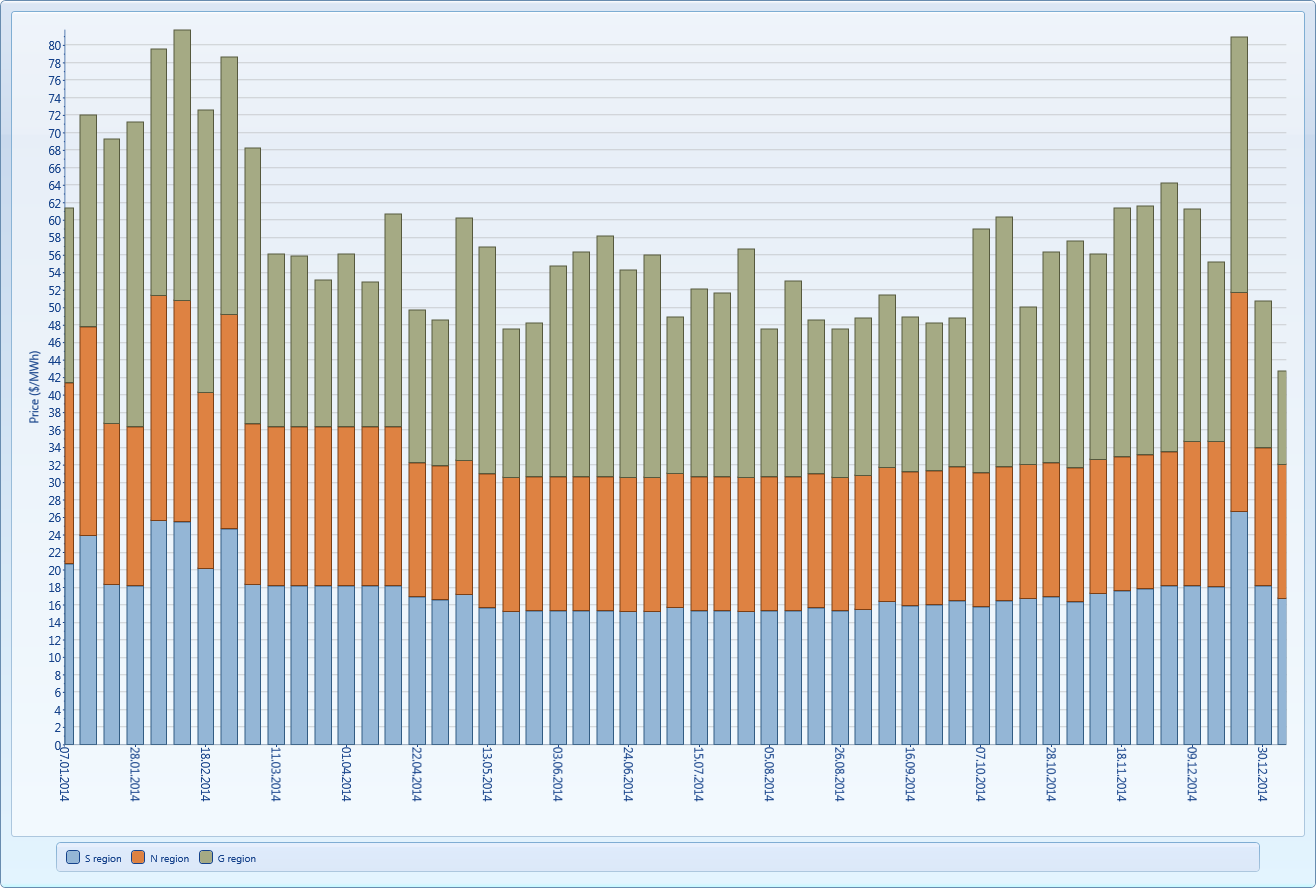
\includegraphics[width=13cm,keepaspectratio=true]{figures/wetcase/MTpriceswet}
\caption{Calculcated prices with high inflow}
\label{fig:MTpriceswet}
\end{center}
\end{figure}
%-------------------------------------------------------------------------------
% expansion planning
%-------------------------------------------------------------------------------
\begin{figure}[htbp]
\begin{center}
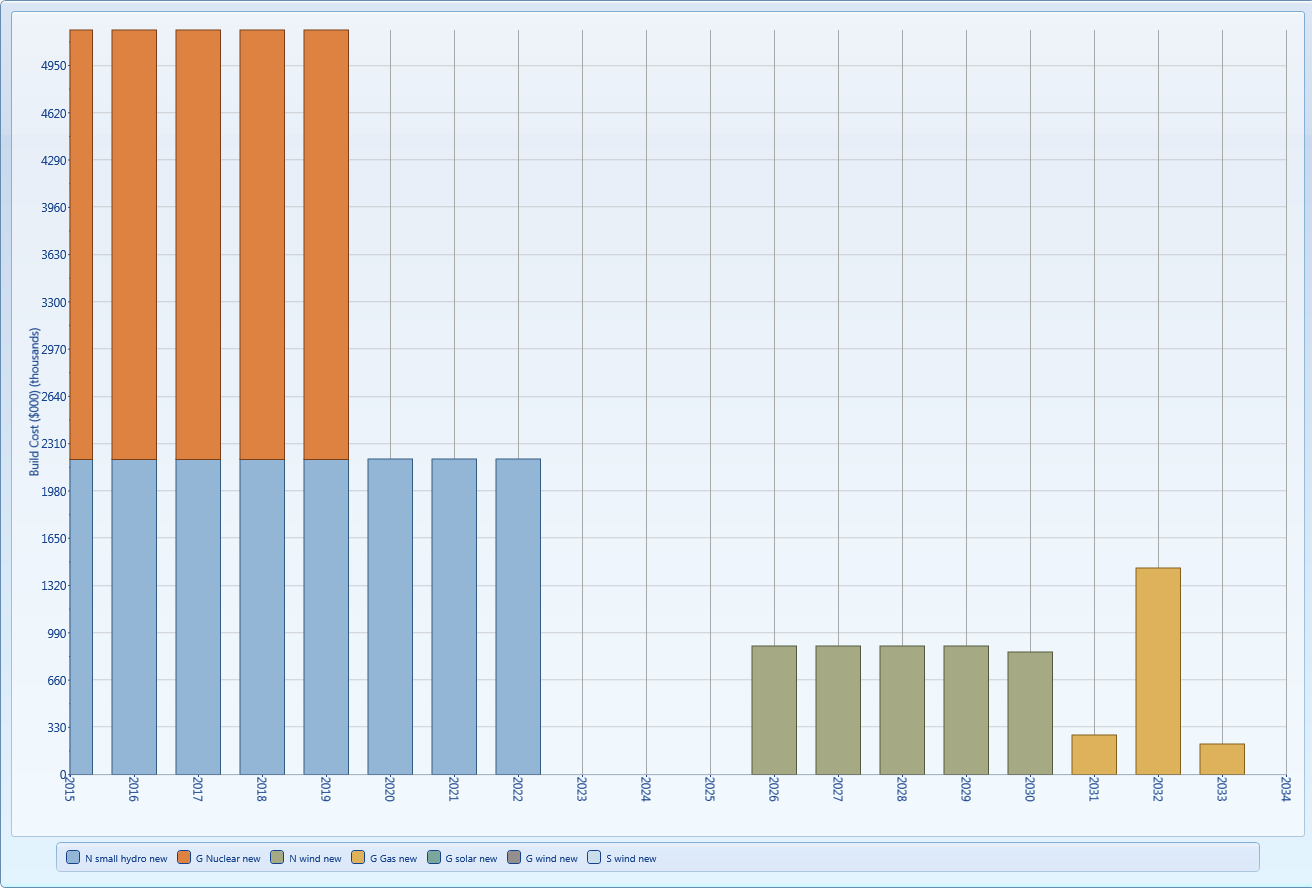
\includegraphics[width=13cm,keepaspectratio=true]{figures/Expansion/EmissionTax/BuildCostET}
\caption{build costs of new generation units using the emission tax system}
\label{fig:BuildCostET}
\end{center}
\end{figure}
\begin{figure}[htbp]
\begin{center}
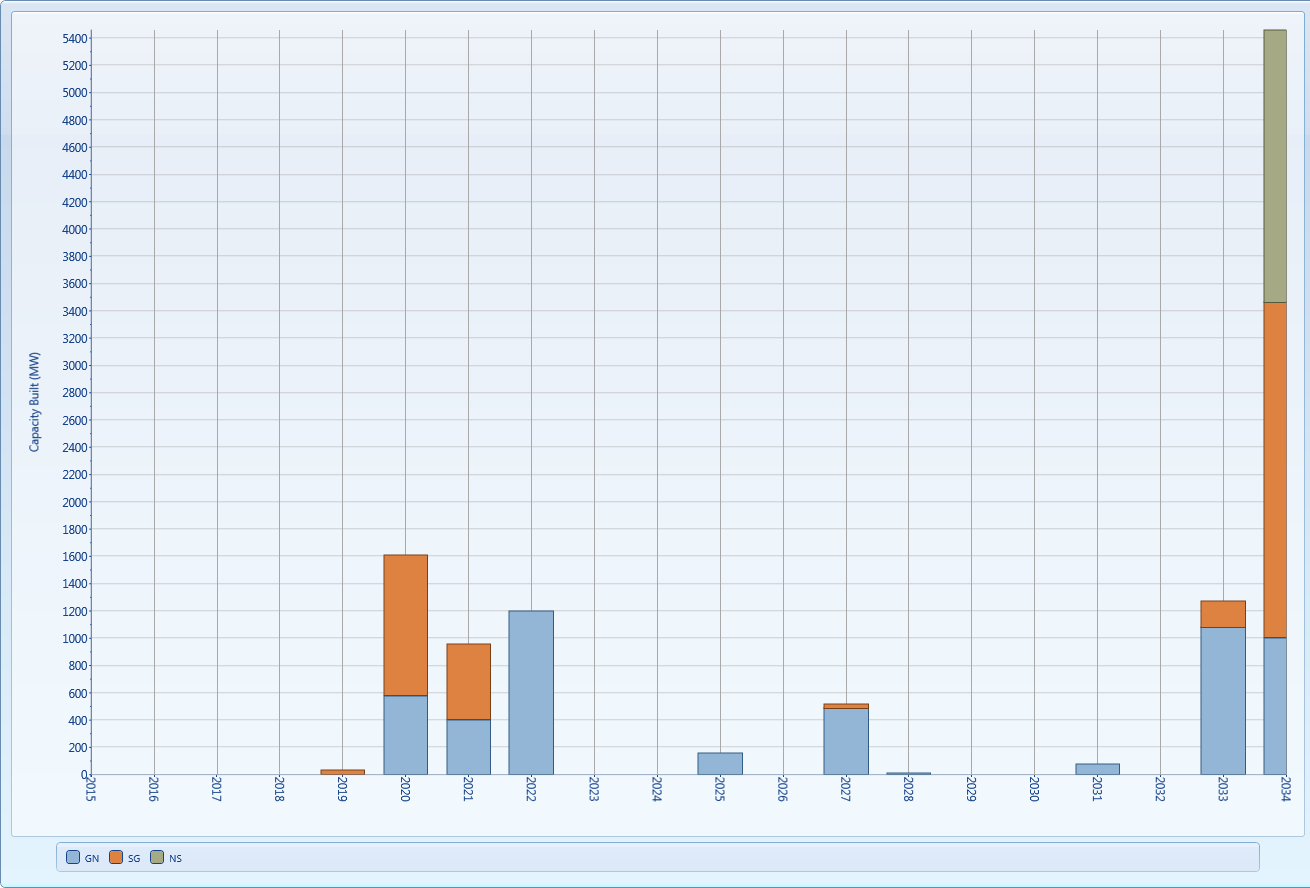
\includegraphics[width=13cm,keepaspectratio=true]{figures/Expansion/EmissionTax/CapacityBuiltInterfaceET}
\caption{interfaces built with emission taxes}
\label{fig:CapacityBuiltInterfaceET}
\end{center}
\end{figure}
\begin{figure}[htbp]
\begin{center}
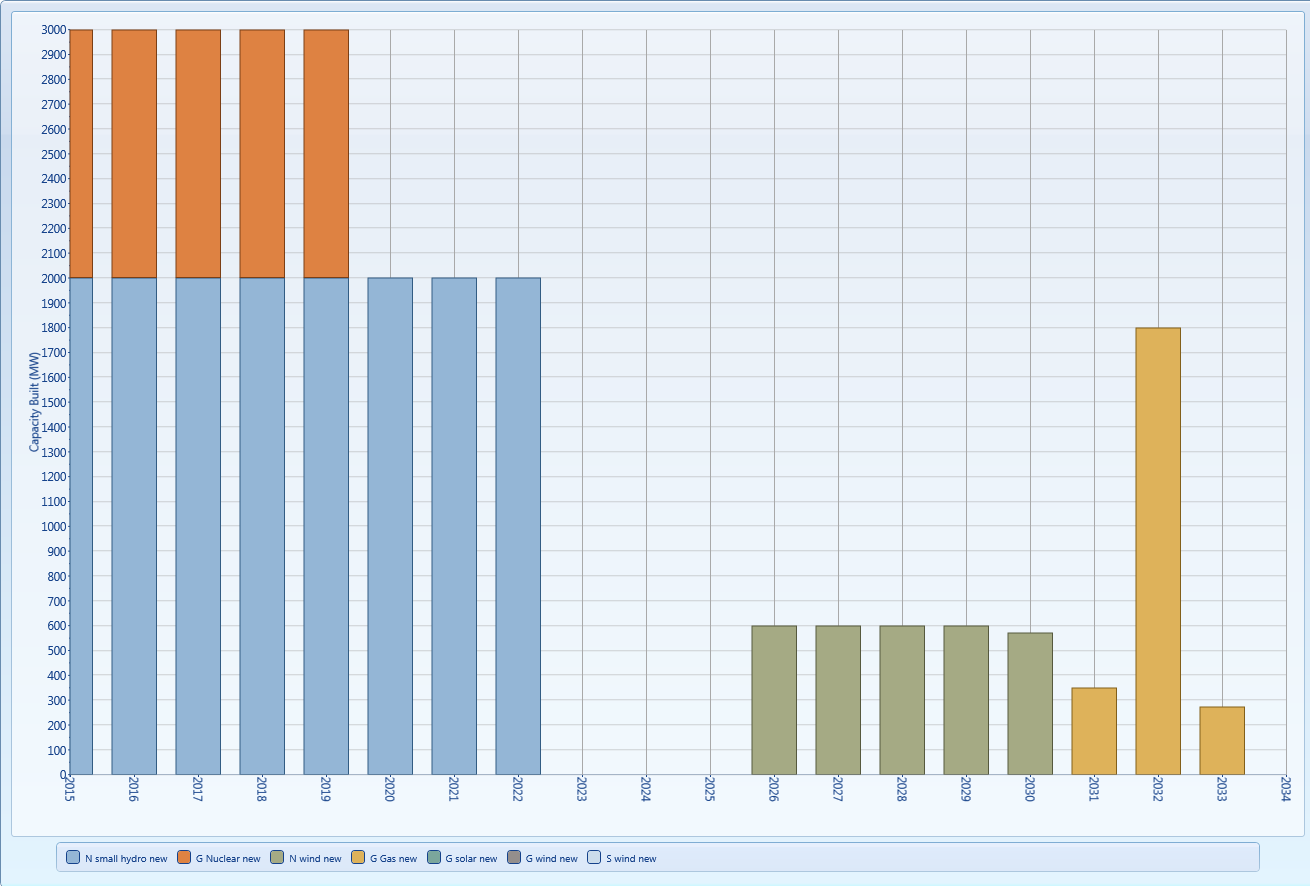
\includegraphics[width=13cm,keepaspectratio=true]{figures/Expansion/EmissionTax/CapacityBuiltNewGenET}
\caption{new generation units when penalized with emission taxes}
\label{fig:CapacityBuiltNewGenET}
\end{center}
\end{figure}
\begin{figure}[htbp]
\begin{center}
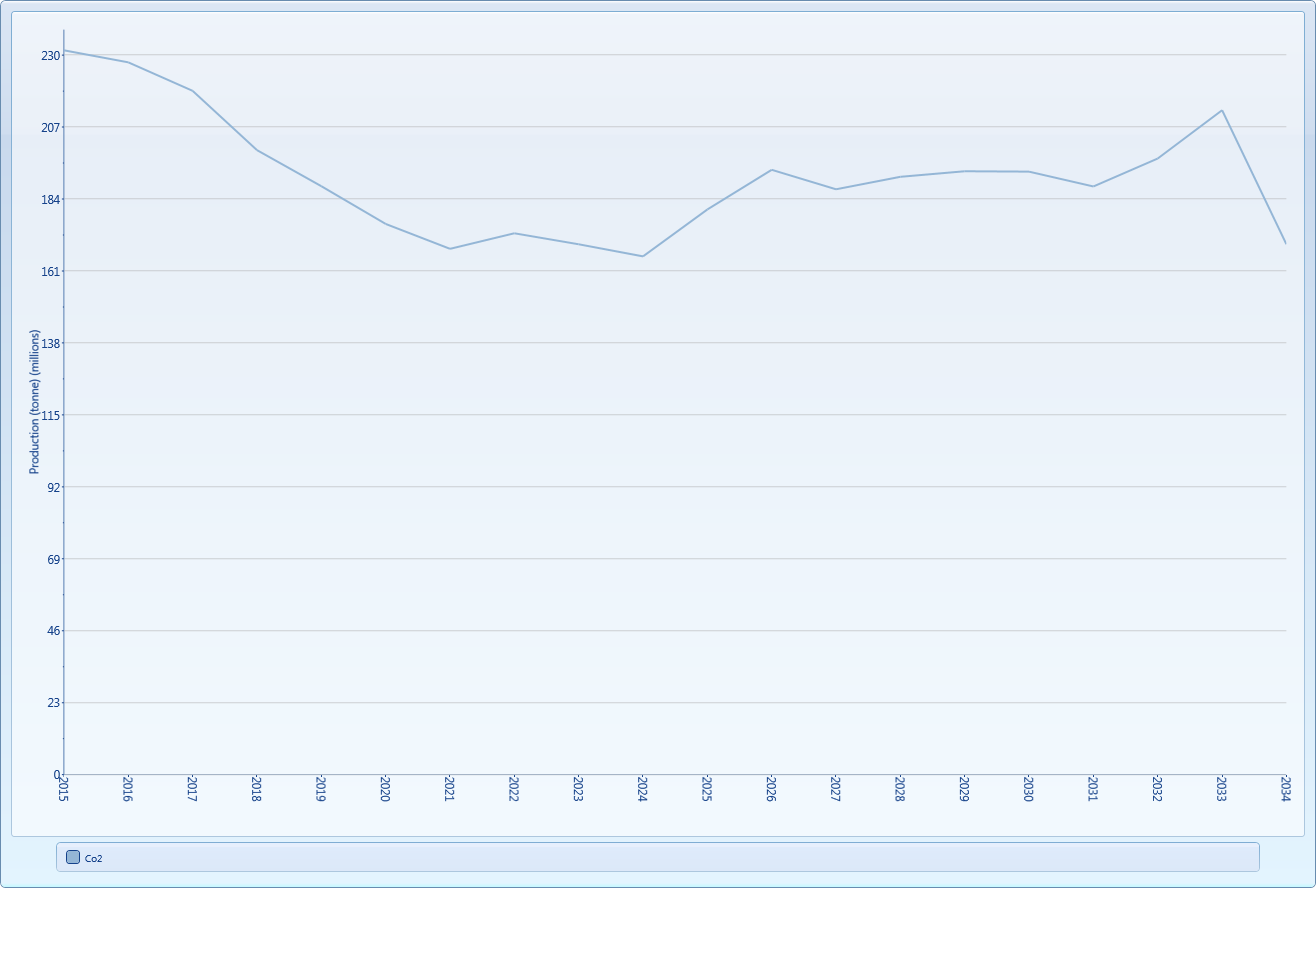
\includegraphics[width=13cm,keepaspectratio=true]{figures/Expansion/EmissionTax/Co2ProductionET}
\caption{emissions with emission tax scheme}
\label{fig:Co2ProductionET}
\end{center}
\end{figure}
\begin{figure}[htbp]
\begin{center}
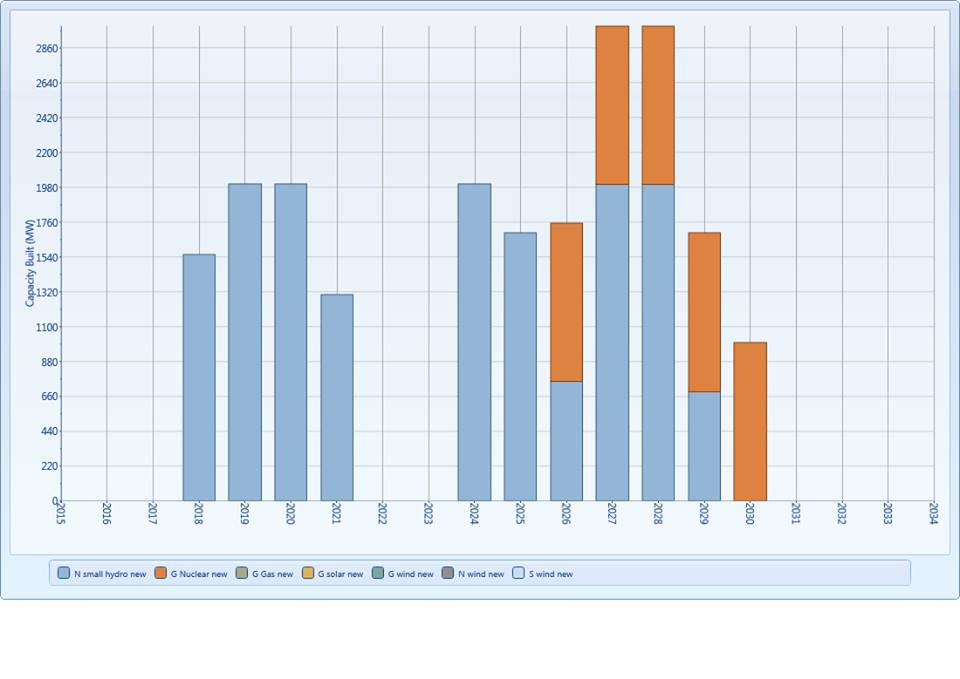
\includegraphics[width=13cm,keepaspectratio=true]{figures/capacitywithout}
\caption{installed capacities without any support}
\label{fig:capacitywithout}
\end{center}
\end{figure}
\begin{figure}[htbp]
\begin{center}
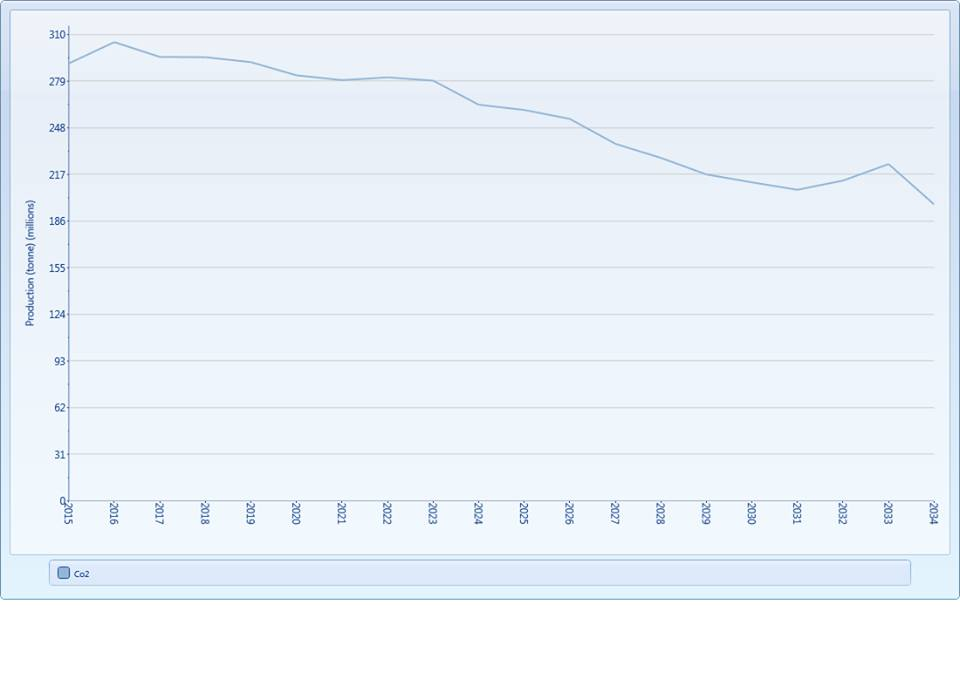
\includegraphics[width=13cm,keepaspectratio=true]{figures/CO2without}
\caption{$CO_2$-emission development at analyzed period without support}
\label{fig:CO2without}
\end{center}
\end{figure}
\end{document}
